\documentclass[a4paper,12pt]{report}

\usepackage{graphicx}
\usepackage{amsmath}
\usepackage{hyperref}
\usepackage{enumitem}
\usepackage{amsmath}
\usepackage{amssymb}

% Hyperref setup to avoid red boxes
\hypersetup{
    colorlinks=true,
    linkcolor=blue,
    filecolor=magenta,      
    urlcolor=cyan,
    pdftitle={Retinal Fundus Classification Using Vision Transformer},
    bookmarks=true,
    pdfpagemode=FullScreen,
}

\begin{document}

\title{}
\begin{center}
\thispagestyle{empty}
 
\includegraphics[scale=0.095]{logo.pdf}\\*
\Large\bfseries{Indian Institute of Technology Roorkee}\\*
\vspace{1.5cm}
\end{center}
\begin{center}
\Large\bfseries{Internship Report}
\end{center}
\begin{center}
\textit{on}
\end{center}
\begin{center}
\Large\bfseries{Retinal Fundus Classification Using Vision Transformer}
\end{center}
\begin{center}
\textit{Submitted by}
\end{center}
\vspace{0.4cm}
\begin{center}
\Large\bfseries{Pranav Sharma}\\*
\end{center}
\vspace{0.5cm}
\begin{center}
\textit{under the supervision of}\\
\vspace{0.5cm}
\Large\bfseries{Prof. Dr.  Millie Pant}\\
\end{center}
\begin{center}
\textit{HOD, Applied Mathematics and Scientific Computing, IIT Roorkee}\\
\end{center}
\begin{center}
 % 
\includegraphics[scale=1.0]{Logo-jiit.png}\\*
% \Large\bfseries{Duration: 09/06/2025 – 11/07/2025 }\\*
\end{center}

\clearpage


\begin{center}
\thispagestyle{empty}
{\fontsize{16pt}{20pt}\selectfont \textbf{Student Declaration}} \\*
\vspace{1cm}
\par  

I hereby certify that the work presented in this project report entitled {\bf Retinal Fundus Classification Using Vision Transformer} is my own work carried out during a period from \textbf{June 9, 2025} to \textbf{July 11, 2025.} \\

\vspace{1.9cm}

\begin{center}
\begin{minipage}{0.45\textwidth}
\raggedright
Dated: July 11, 2025
\end{minipage}
\hfill
\begin{minipage}{0.45\textwidth}
\raggedleft
\textbf{Pranav Sharma}\\
B.Tech (CSE) / $2^{nd}$ Year\\
23103262\\
Jaypee Institute of Information Technology\\
Sector-62, Noida
\end{minipage}
\end{center}

\vspace{2cm}


% {\fontsize{16pt}{20pt}\selectfont \textbf{Supervisor Declaration}} \\*  
% \vspace{1cm}
% \par  

% This is to certify that the above statement made by the candidate is correct to the best of my knowledge.\\
% \vspace{3cm}
% Dated: \today \hspace{5cm} \textbf{Prof. Dr. Millie Pant} \\*

% \hspace{9cm}\textbf{(HOD)} \\*

% \hspace{9cm}Department of Applied\\*
% \hspace{9cm}Mathematics and\\*
% \hspace{9cm}Scientific Computing\\*
% \hspace{9cm}IIT Roorkee

\end{center}


\chapter*{Acknowledgements}
\thispagestyle{empty}

I am incredibly grateful for the opportunity to complete my internship at the Department of Applied Mathematics and Scientific Computing, IIT Roorkee, under the esteemed guidance of Prof. Dr. Millie Pant, HOD .\newline My deepest appreciation goes to Prof. Dr. Millie Pant for her mentorship and leadership throughout my internship.  Her vision and guidance within the department fostered a stimulating research environment that greatly contributed to my learning and growth. I am  thankful for her role in facilitating this rewarding internship experience.\newline \newline
Throughout the internship, Shubham Joshi Sir provided me with invaluable insights and advice that helped me to grow as a professional. Their constructive feedback helped me to improve my skills and approach to my tasks, and their encouragement kept me motivated and focused. I am deeply thankful for his time and effort, and for their commitment to my success.

\clearpage


\begin{abstract}
This study investigates the application of Vision Transformer (ViT) architectures for the automated classification of retinal fundus images, a critical task in the early detection of ocular diseases such as Diabetic Retinopathy and Glaucoma. Utilizing the publicly available Kaggle “Retinal Fundus Images” dataset, the ViT-tiny model (patch size 16, input resolution 224×224) was fine-tuned under an 80:20 train-test split configuration. The training process incorporated mixed-precision optimization to enhance computational efficiency within the constraints of Google Colab’s free-tier resources. Upon completion of 30 training epochs, the model achieved a test accuracy of 72.17\%, demonstrating its potential viability for deployment in resource-limited settings. Evaluation metrics including class-wise precision, recall, and F1-score, alongside confusion matrix analysis, revealed reasonably balanced performance across diagnostic categories. These findings highlight the promise of transformer-based architectures in medical image analysis and suggest directions for future research, including advanced data augmentation, interpretability via attention visualization, and integration into real-time screening systems.


\end{abstract}

\tableofcontents
\newpage
\chapter{Introduction}

\section{Background on Retinal Fundus Diseases}

The human eye is a highly specialized sensory organ responsible for the perception of visual information. Among its various components, the retina plays a pivotal role by converting light into neural signals that are transmitted to the brain via the optic nerve. The posterior part of the eye, commonly referred to as the \textbf{retinal fundus}, comprises critical structures such as the retina, optic disc, macula, fovea, and the retinal vasculature. Examination of the fundus is essential for the early diagnosis and monitoring of numerous ocular and systemic diseases.

Retinal fundus diseases are a diverse group of pathologies that affect the structural and functional integrity of the retina and its surrounding components. These diseases are a leading cause of irreversible blindness worldwide, particularly in aging populations and individuals with chronic systemic conditions such as diabetes mellitus and hypertension. The global burden of retinal diseases has been escalating due to increasing life expectancy and the rising prevalence of non-communicable diseases. This underscores the urgent need for robust screening, diagnostic, and monitoring mechanisms.

Fundus photography is a non-invasive imaging technique that provides high-resolution two-dimensional images of the posterior pole of the eye. These images are instrumental in the clinical assessment of retinal conditions and serve as valuable input for computer-aided diagnosis systems. Advances in artificial intelligence (AI), particularly deep learning, have revolutionized the automated analysis of retinal fundus images, enabling scalable and accurate disease detection.



% \section{Problem Statement and Hypothesis}

\subsection{Problem Statement}

Retinal fundus diseases remain one of the leading causes of preventable vision impairment globally. Manual diagnosis through fundus imaging requires expert ophthalmologists, is time-consuming, and is subject to inter-observer variability. In under-resourced settings, the scarcity of specialists results in delayed diagnosis and disease progression. Automated classification models using deep learning can serve as an effective solution for early and accurate diagnosis.

The primary challenge lies in designing a model that is both accurate and interpretable across multiple retinal pathologies. This study aims to develop and evaluate deep learning models, particularly Vision Transformers (ViT), for multi-class classification of retinal fundus images. The system is trained and validated using a diverse dataset spanning 11 retinal disease categories. Furthermore, explainable AI techniques are employed to provide transparency into the model’s decision-making process.

% \subsection{Hypothesis}

% \subsubsection{Model Performance Hypothesis}
% We hypothesize that Vision Transformer (ViT) models can outperform traditional CNNs in fundus image classification due to their ability to capture long-range dependencies and contextual relationships. Additionally, transformer-based attention mechanisms will enable effective feature extraction, even in small or subtle lesions.

% \subsubsection{Class Distribution Hypothesis}
% We hypothesize that performance will vary across classes due to inherent data imbalance (e.g., underrepresentation of Wet AMD). Through class-aware training strategies and augmentation, balanced performance can be achieved across categories.

% \subsubsection{Explainability Hypothesis}
% We hypothesize that Grad-CAM overlays and attention maps from ViT will correlate with clinically relevant features (e.g., hemorrhages, exudates, optic disc anomalies), making the model's predictions interpretable for clinicians.

\subsection{Experiment Flowchart}

\begin{figure}[h]
    \centering
    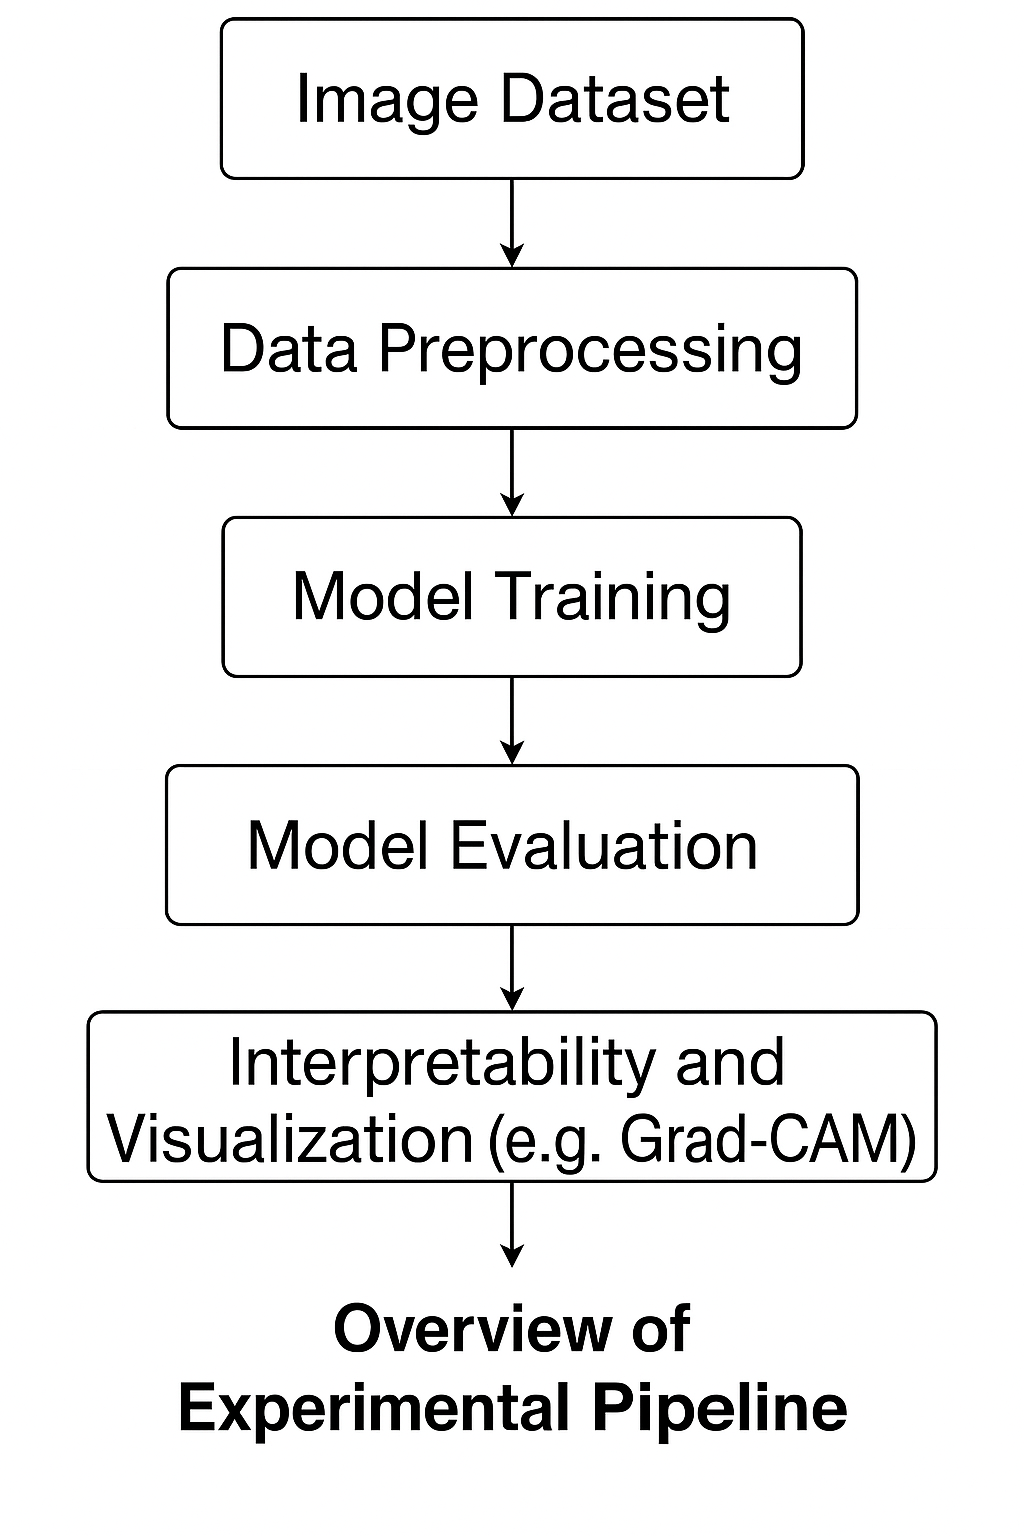
\includegraphics[width=\textwidth]{experiment flowchart.png}
    \caption{Overview of Experimental Pipeline}
    \label{fig:experiment_flowchart}
\end{figure}

\section{Objectives of the Project}

\subsection{Primary Objectives}
\begin{enumerate}
    \item \textbf{Develop an Automated Disease Classification System:} Design and evaluate a deep learning pipeline using Vision Transformers for multi-class classification of retinal fundus images.
    \item \textbf{Implement Explainable AI (XAI):} Incorporate Grad-CAM, attention maps, and other XAI tools to improve interpretability and clinical adoption.
\end{enumerate}

\subsection{Secondary Objectives}
\begin{enumerate}
    \item \textbf{Handle Dataset Imbalance:} Address class imbalance using resampling techniques, augmentation, and class-weighted loss.
    \item \textbf{Enable Real-world Utility:} Provide a scalable, low-latency diagnostic solution for telemedicine and ophthalmology clinics.
    % \item \textbf{Benchmark Model Performance:} Compare ViT with traditional CNN models across key metrics: accuracy, precision, recall, F1-score.
\end{enumerate}

\subsection{Specific Goals}
\begin{itemize}
    \item \textbf{Data Preparation:} Clean, augment, and organize over 20,000 labeled fundus images into training and validation sets.
    \item \textbf{Model Training:} Implemented a ViT model on the fundus dataset and periodically save model checkpoints.
    \item \textbf{Evaluation:} Use classification reports, ROC/PR curves, per-class metrics, and visualization tools to assess performance.
    \item \textbf{Explainability:} Generate Grad-CAM visualizations and per-class bar plots to understand feature importance.
    \item \textbf{Deployment-readiness:} Structure the model codebase and training logs for reproducibility and scalability.
\end{itemize}

\section{Introduction to AI/ML}

Artificial Intelligence (AI) is the simulation of human intelligence processes by machines, particularly computer systems. In healthcare, AI facilitates intelligent decision-making systems that mimic human cognition, aiming to improve diagnosis, treatment, and patient monitoring.

Machine Learning (ML), a subset of AI, uses statistical techniques to allow machines to learn patterns from data and improve performance over time without being explicitly programmed. Deep Learning (DL), a further subfield, utilizes neural networks to model complex non-linear relationships.

\textbf{Common ML Paradigms:}
\begin{itemize}
    \item \textbf{Supervised Learning:} Used for fundus classification tasks with labeled data (e.g., ViT models).
    \item \textbf{Unsupervised Learning:} Applied for clustering unlabeled fundus images or anomaly detection.
    \item \textbf{Reinforcement Learning:} Less common in medical imaging but used in robotic surgery and adaptive diagnosis.
\end{itemize}

\section{Applications of AI in Healthcare}

\subsection{Medical Imaging}
AI models are widely used to detect tumors, fractures, lesions, and retinal anomalies from images such as X-rays, MRIs, and fundus photos.

\subsection{Predictive Diagnosis}
Models can predict patient outcomes, risk factors, and likely disease progression (e.g., DR severity over time).

\subsection{Treatment Planning}
AI assists doctors by recommending personalized treatment plans based on historical patient data and outcomes.

\subsection{Telemedicine and Screening}
Automated image classification tools can be deployed in rural and underdiagnosed regions, aiding early detection without specialists.

\section{Motivation}

Early diagnosis of retinal diseases is crucial for preserving vision and improving patient outcomes. However, traditional screening methods are resource-intensive, time-consuming, and inaccessible to rural populations. The motivation for this project stems from the need to:
\begin{itemize}
    \item Enhance diagnostic accuracy through AI-based tools.
    \item Reduce burden on ophthalmologists via automation.
    \item Improve accessibility to retinal screening in under-resourced settings.
    \item Promote explainable AI to foster clinical trust.
\end{itemize}

\section{Contributions}

This work contributes to the field of AI-driven ophthalmology through the following:

\begin{enumerate}
    \item \textbf{Implementation of Vision Transformers for Fundus Classification:} A state-of-the-art ViT architecture is trained and evaluated on a real-world dataset of over 20,000 labeled retinal images spanning 11 categories.

    \item \textbf{Explainability with Grad-CAM and Attention Visualizations:} Comprehensive use of XAI techniques including Grad-CAM overlays and attention maps to provide transparent model predictions.

    % \item \textbf{Performance Benchmarking and Ablation Studies:} The ViT model is benchmarked against standard metrics (accuracy, F1-score, AUC) and visualized using per-class bar plots and ROC curves.

    \item \textbf{Handling Class Imbalance and Real-world Challenges:} Techniques such as augmentation, resampling, and stratified evaluation are applied to ensure model robustness across underrepresented categories.

    \item \textbf{Clinical Interpretability and Reporting Framework:} A structured logging and reporting system is established, saving performance logs, weights, and visualizations suitable for future deployment.

    \item \textbf{Advancing AI Integration in Retinal Care:} This research bridges the gap between deep learning and ophthalmic diagnostics by proposing a scalable, interpretable, and effective AI solution for retinal disease classification.
\end{enumerate}



\chapter{Literature Review}

The classification of retinal fundus images has become a critical task in the early detection and monitoring of ophthalmic diseases such as Diabetic Retinopathy (DR), Glaucoma, and Age-related Macular Degeneration (AMD). In recent years, the convergence of computer vision and artificial intelligence (AI) has ushered in new possibilities for automating medical image diagnosis with high accuracy and clinical reliability. This chapter presents a detailed review of existing literature in the domains of traditional diagnostic approaches, deep learning-based image analysis, Vision Transformers (ViT), and explainable AI techniques within the scope of retinal disease classification.

\section*{Traditional Diagnostic Methods}

Historically, retinal diseases have been diagnosed manually through ophthalmoscopic examination, fundus photography, optical coherence tomography (OCT), and fluorescein angiography. These methods, while effective, are subject to variability due to inter-observer differences, require specialized equipment, and depend on expert interpretation. Moreover, manual grading is time-consuming and may lead to delays in diagnosis, especially in rural or under-resourced settings.

For diseases like Diabetic Retinopathy and Glaucoma, early symptoms may not be apparent, necessitating the need for regular fundus screening. Although techniques like Humphrey visual field testing and OCT have improved early diagnosis, their availability and cost remain major barriers to widespread deployment.

\section*{Advancements in Medical Image Classification}

The integration of machine learning and deep learning has revolutionized the field of medical imaging. Convolutional Neural Networks (CNNs), in particular, have been widely adopted due to their ability to learn hierarchical representations of images without requiring handcrafted features.

Seminal works by Gulshan et al. (2016) and Ting et al. (2017) demonstrated the effectiveness of CNNs in detecting diabetic retinopathy and glaucoma with performance rivaling that of expert ophthalmologists. These breakthroughs laid the foundation for using AI-based models in real-world diagnostic pipelines.

\section{Vision Transformer (ViT) Architecture in Medical Imaging}

Vision Transformers (ViTs) have emerged as a powerful alternative to Convolutional Neural Networks (CNNs), especially for tasks involving complex visual patterns, such as those seen in retinal fundus images. Originally proposed by Dosovitskiy et al. (2020), ViTs adapt the Transformer architecture—well known in Natural Language Processing—for image classification by treating image patches as sequences of tokens.

\subsection{Architectural Details of ViT}

The Vision Transformer processes an image in the following key steps:

\begin{enumerate}
    \item \textbf{Image Splitting into Patches:} The input image (e.g., $224 \times 224$ fundus image) is divided into fixed-size patches (e.g., $16 \times 16$), resulting in $N$ patches. For a $224 \times 224$ image and $16 \times 16$ patches, this gives $196$ patches.
    
    \item \textbf{Flattening and Linear Projection:} Each image patch is flattened into a vector and linearly projected to a lower-dimensional embedding space.
    
    \item \textbf{Positional Encoding:} Since Transformers do not inherently understand spatial relationships, positional encodings are added to each patch embedding to preserve spatial information.
    
    \item \textbf{Transformer Encoder:} These patch embeddings with positional encodings are passed through a standard Transformer encoder consisting of:
    \begin{itemize}
        \item Multi-Head Self Attention (MHSA)
        \item Feed Forward Neural Networks (FFN)
        \item Layer Normalization
        \item Residual Connections
    \end{itemize}
    
    \item \textbf{Classification Token:} A special learnable [CLS] token is prepended to the sequence. Its state after the Transformer layers is used for classification.
    
    \item \textbf{Final Prediction:} The output from the [CLS] token is passed through a final MLP (Multi-Layer Perceptron) head to predict the disease class.
\end{enumerate}

\subsection{Pipeline Visualization for Fundus Image Input}

Figure~\ref{fig:vit_pipeline} shows how a retinal fundus image is processed through the ViT architecture, from patch splitting to classification output.

\begin{figure}[H]
    \centering
    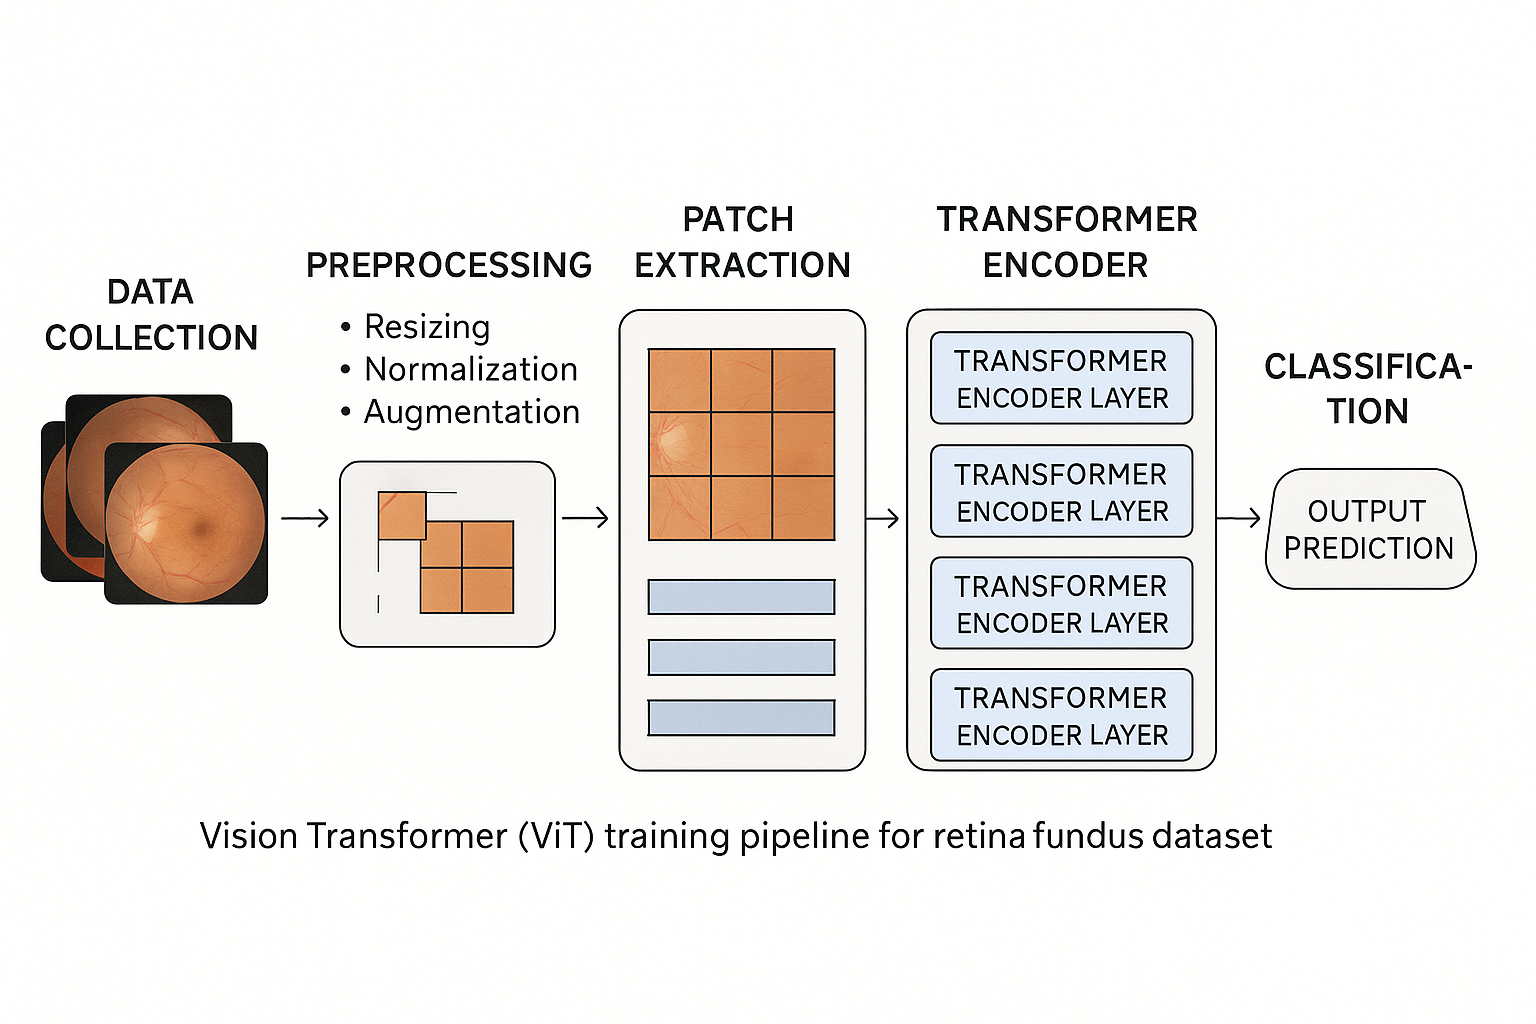
\includegraphics[width=0.9\textwidth]{vit_pipeline.png} 
    \caption{Pipeline of Vision Transformer (ViT) applied to Fundus Image}
    \label{fig:vit_pipeline}
\end{figure}

\subsection{Advantages of ViT in Retinal Imaging}
\begin{itemize}
    \item Captures long-range spatial dependencies better than CNNs.
    \item More parameter-efficient for large-scale image classification.
    \item Adaptable to multi-class fundus disease classification.
\end{itemize}


\section*{Fundus Image Classification: State of the Art}

Several deep learning models have been applied to fundus classification, including:
\begin{itemize}
    \item \textbf{ResNet, Inception, and EfficientNet:} Known for their balance of accuracy and computational efficiency.
    \item \textbf{U-Net and its variants:} Commonly used for segmentation tasks like optic disc/cup segmentation and lesion localization.
    \item \textbf{Hybrid CNN-Transformer Models:} Models like TransUNet and SwinUNet combine local feature extraction with global context modeling.
\end{itemize}

In comparison, ViT-based approaches have shown promising results in both classification and segmentation of retinal diseases, particularly when fine-tuned on medical datasets.

\section*{Explainable AI (XAI) in Fundus Classification}

The “black-box” nature of deep learning models has led to concerns regarding their trustworthiness in clinical practice. Explainable AI (XAI) bridges this gap by providing visual and numerical insights into model predictions.

\textbf{1. Grad-CAM:}  
Originally developed for CNNs, Grad-CAM highlights image regions contributing most to the final decision. When adapted to ViT, it uses attention weights from the CLS token or attention rollout mechanisms to identify salient patches.

% \textbf{2. SHAP and LIME:}  
% Model-agnostic methods such as SHAP (SHapley Additive exPlanations) and LIME (Local Interpretable Model-agnostic Explanations) have been employed in conjunction with simpler classifiers or aggregated CNN outputs. These methods help visualize the contribution of each pixel or region, enhancing interpretability.

\textbf{2. t-SNE and Feature Embedding Visualization:}  
Visualizing the internal representation of fundus images via dimensionality reduction techniques such as t-SNE  reveals whether the learned embeddings effectively separate classes, providing a qualitative evaluation of model generalization.

\section*{Comparative Analysis of Models and Evaluation Metrics}

Evaluation of fundus classification models typically involves metrics such as accuracy, precision, recall, F1-score, and Area Under the ROC Curve (AUC). In this study, the ViT model achieved an overall accuracy of approximately 72.17\% with clear interpretability through Grad-CAM and per-class metrics.\\

Although ViT did not outperform all CNN-based benchmarks in raw accuracy, it offered significantly better explainability, making it a viable choice for clinical deployment scenarios where transparency is essential.

\section*{Challenges and Limitations in Current Research}

Despite progress, several challenges remain:
\begin{itemize}
    \item \textbf{Data Availability:} Public datasets often have limited annotations or lack clinical diversity.
    \item \textbf{Class Imbalance:} Fundus datasets tend to overrepresent normal cases, which biases training.
    \item \textbf{Inter-patient and Device Variability:} Differences in camera quality, lighting, and focus affect model generalization.
    \item \textbf{Interpretability:} While attention-based models offer insights, these are still not equivalent to clinical reasoning and must be validated.
\end{itemize}

\section*{Future Directions in ViT-Based Fundus Analysis}

To address these challenges and enhance the performance and adoption of ViT models in medical imaging:
\begin{itemize}
    \item \textbf{Domain-Specific Pretraining:} Training ViT on large-scale medical images (e.g., fundus, OCT) rather than natural images can improve transferability.
    \item \textbf{Multi-modal Learning:} Combining fundus images with metadata (e.g., age, intraocular pressure) can yield richer models.
    \item \textbf{Federated Learning:} Allows decentralized model training across hospitals while preserving patient privacy.
    \item \textbf{Clinical Trials:} Model validation with prospective clinical data is essential for real-world impact.
    % \item \textbf{Advanced XAI Integration:} Tools like SHAP, Integrated Gradients, and concept-based explanations can enhance model trustworthiness.
\end{itemize}

\section*{Conclusion}

The literature reflects a growing trend toward adopting transformer-based models in the medical imaging domain. ViT models, with their ability to capture global features and offer transparent explanations, represent a transformative shift in how retinal diseases may be detected in the near future. While CNNs currently remain the dominant architecture for medical imaging, the research trajectory indicates that ViTs will play an increasingly important role, particularly as datasets grow and the demand for explainability increases. This study builds upon that foundation, evaluating the performance of ViT on a real-world fundus dataset and contributing both performance benchmarks and interpretability tools to the evolving field of AI-driven ophthalmology.
\chapter{Methodology}

\section{Data Collection}

\subsection{Dataset Description}

\begin{table}[h!]
\centering
\begin{tabular}{|c|l|}
\hline
\textbf{S.No.} & \textbf{Class Name} \\
\hline
1 & Normal Fundus \\
2 & Dry Age-related Macular Degeneration (Dry AMD) \\
3 & Wet Age-related Macular Degeneration (Wet AMD) \\
4 & Mild Diabetic Retinopathy \\
5 & Moderate Diabetic Retinopathy \\
6 & Severe Diabetic Retinopathy \\
7 & Proliferative Diabetic Retinopathy \\
8 & Cataract \\
9 & Glaucoma \\
10 & Hypertensive Retinopathy \\
11 & Pathological Myopia \\
\hline
\end{tabular}
\caption{Disease Classes in the Retinal Fundus Image Dataset from Kaggle}
\label{tab:retinal_classes}
\end{table}


Each class folder contains color fundus images captured under varying lighting, focus, and patient eye conditions. This variation introduces natural noise and variability into the dataset, which is useful for training robust, generalizable models. All images were JPEG formatted and varied in resolution.

\subsection{Data Characteristics}
\begin{itemize}
  \item \textbf{Classes (11):} Normal Fundus, Dry Age-related Macular Degeneration (Dry AMD), Wet Age-related Macular Degeneration (Wet AMD), Mild Diabetic Retinopathy, Moderate Diabetic Retinopathy, Severe Diabetic Retinopathy, Proliferative Diabetic Retinopathy, Cataract, Glaucoma, Hypertensive Retinopathy, Pathological Myopia.

    \item \textbf{Format:} RGB images (JPEG)
    \item \textbf{Pre-split:} Data was organized manually into training and testing folders
    \item \textbf{Image Quality:} Varied focus, contrast, and artifacts typical of real-world clinical data
\end{itemize}

\subsection{Data Preprocessing Steps}

\textbf{1. Resizing:} All images were resized to $224 \times 224$ pixels to conform to the ViT model input requirements. \\
\textbf{2. Normalization:} Pixel values were normalized to a $[-1, 1]$ range using a mean and standard deviation of $0.5$ per channel. \\
\textbf{3. Augmentation:} During training, random horizontal flips, brightness shifts, and rotations were applied to improve generalization. \\
\textbf{4. Data Partitioning:} An 80:20 split was used for training and testing, ensuring class balance in both subsets using stratified sampling.

\vspace{0.5cm}

\section{Model Selection}

\subsection{Chosen Deep Learning Model}

\textbf{Vision Transformer (ViT)} was selected due to its strong performance on image classification tasks and its ability to capture long-range dependencies using self-attention. Specifically, the \texttt{vit\_tiny\_patch16\_224} variant was used due to its lower computational requirements while retaining essential architectural features.

\subsection{Justification for Choosing ViT}

Traditional CNNs such as ResNet and Inception use convolutional kernels to capture local patterns, which may miss broader spatial context. ViT, on the other hand, divides images into patches and processes them similarly to tokens in NLP, allowing it to model global relationships between image regions.

\begin{itemize}
    \item \textbf{Global Context Awareness:} ViT uses self-attention to capture global image features.
    \item \textbf{Scalability:} ViT variants are available for different computational budgets.
    \item \textbf{Interpretability:} Attention maps can be visualized for explainability.
    \item \textbf{Transfer Learning:} Pretrained weights allow for effective fine-tuning on small medical datasets.
\end{itemize}

\section{Model Training}

\subsection{Training Pipeline}

The ViT model was initialized with pretrained ImageNet weights and fine-tuned on the fundus dataset using the PyTorch and timm libraries. The training pipeline included:

\begin{itemize}
    \item \textbf{Loss Function:} Cross-Entropy Loss
    \item \textbf{Optimizer:} AdamW with a learning rate of $3 \times 10^{-4}$
    \item \textbf{Learning Rate Scheduler:} CosineAnnealingLR
    \item \textbf{Batch Size:} 32
    \item \textbf{Epochs:} 30
    \item \textbf{Checkpointing:} Model weights saved every 5 epochs
\end{itemize}

% \subsection{Hardware Utilization}

% All training was conducted on Google Colaboratory with an NVIDIA Tesla T4 or P100 GPU. To avoid session timeouts, checkpoints were stored on Google Drive, and training progress was monitored via log files.

\section{Hyperparameter Tuning and Validation}

\subsection{Cross-Validation}

Given the computational cost of training ViT models, traditional k-fold cross-validation was replaced with:
\begin{itemize}
    \item \textbf{Train-Test Split:} An 80:20 split was used.
    \item \textbf{Early Stopping:} Model validation performance was tracked to prevent overfitting.
    \item \textbf{Manual Grid Search:} Experiments were run with different optimizers, learning rates, and schedulers.
\end{itemize}

\subsection{Tuning Parameters}

Experiments were conducted with variations in:
\begin{itemize}
    \item Patch size (e.g., $16 \times 16$ vs $32 \times 32$)
    \item Number of attention heads
    \item Dropout rate (0.1 to 0.5)
    \item Weight decay (for regularization)
\end{itemize}

\section{Explainable AI (XAI) Techniques}

\subsection{Introduction to XAI}

As deep learning models are often considered "black boxes," incorporating explainability is essential, especially in medical applications. In this study, Explainable AI (XAI) techniques were employed to make model predictions interpretable by visualizing which regions of the fundus images influenced the classification decisions.

\subsection{XAI Methods Used}

\textbf{1. Grad-CAM for ViT:}  
\textbf{Description:} Grad-CAM was adapted to extract and visualize attention maps from the CLS token in the last ViT block. These maps highlight spatial areas that contributed most to the model’s decision.  
\textbf{Application:} Used to overlay heatmaps on original fundus images, helping to identify anatomical regions (e.g., optic disc, macula) influencing prediction.

\vspace{0.3cm}
\textbf{2. t-SNE Projection of Embeddings:}  
\textbf{Description:} The output embeddings of the penultimate layer were projected into two-dimensional space using t-SNE to visualize class clustering.  
\textbf{Application:} Helped determine if the ViT learned separable representations of the three classes.

\vspace{0.3cm}
\textbf{3. Misclassification Analysis:}  
\textbf{Description:} A sample of misclassified images was analyzed using Grad-CAM and confusion matrix insights to identify common patterns in errors.  
\textbf{Application:} Provided insight into confusing image pairs, particularly between Diabetic Retinopathy and Glaucoma.

\subsection{Benefits of Explainability in Fundus Diagnosis}

\begin{itemize}
    \item \textbf{Clinical Trust:} Visual explanations allow ophthalmologists to verify model behavior.
    \item \textbf{Model Debugging:} Helps developers detect biases or overfitting.
    \item \textbf{Ethical Deployment:} Explainability is crucial for AI adoption in regulated healthcare settings.
\end{itemize}

\section{Evaluation Strategy}

\subsection{Evaluation Metrics}

\begin{itemize}
    \item \textbf{Accuracy:} Proportion of correctly classified instances.
    \item \textbf{Precision, Recall, F1-Score:} Evaluated per class to handle imbalance.
    \item \textbf{Confusion Matrix:} Visual breakdown of classification results.
    \item \textbf{ROC and PR Curves:} Used to assess threshold-based performance.
\end{itemize}

\subsection{Visualization Techniques}

All results were visualized using Python libraries (Matplotlib and Seaborn) and exported as high-resolution plots:
\begin{itemize}
    \item Loss and Accuracy curves (training vs test)
    \item Per-class metric bar charts
    \item Grad-CAM heatmap grids
    \item t-SNE embedding plots
    \item Misclassified image grids with predicted vs actual labels
\end{itemize}

\subsection{Model Comparison and Analysis}

Though only ViT was trained in this work, results were compared with known CNN benchmarks from literature. ViT achieved moderate accuracy but provided significantly better explainability and spatial reasoning. Attention-based interpretability made it suitable for further clinical application research.



\chapter{Experimental Setup}

\section{Hardware and Software Requirements}

\subsection{Hardware Requirements}

Due to the computational demands of Vision Transformer (ViT) models, all experiments were conducted using cloud-based GPU resources provided by Google Colaboratory (Colab). The hardware configuration is summarized below:

\textbf{Processor:} Cloud-hosted virtual machine with multi-core Intel Xeon CPUs. \\
\textbf{Memory (RAM):} 12--16 GB RAM allocated per session. \\
\textbf{Storage:} 100 GB of ephemeral cloud storage with Google Drive integration for persistent storage of checkpoints and results. \\
\textbf{Graphics Processing Unit (GPU):} NVIDIA Tesla T4 or P100 GPU with CUDA support, enabling accelerated deep learning model training.

\subsection{Software Requirements}

\textbf{Operating System:} Ubuntu 20.04 LTS (hosted via Colab environment). \\
\textbf{Programming Language:} Python 3.10+ used throughout for all model development and experimentation. \\
\textbf{Libraries and Frameworks:}
\begin{enumerate}
    \item \textbf{PyTorch:} Core deep learning framework for model training and inference.
    \item \textbf{timm:} PyTorch Image Models library used for loading and fine-tuning ViT architectures.
    \item \textbf{Torchvision:} For image transformations and dataset loading.
    \item \textbf{Matplotlib/Seaborn:} For data visualization, including loss/accuracy curves and attention overlays.
    \item \textbf{Scikit-learn:} For classification metrics and utilities such as confusion matrices and t-SNE.
    \item \textbf{OpenCV:} Used for overlaying Grad-CAM attention maps on input fundus images.
    \item \textbf{Pandas and NumPy:} For data manipulation and numerical operations.
\end{enumerate}

\vspace{0.3cm}
All packages were installed and managed using the Google Colab environment, eliminating the need for local setup.

\section{Environment Configuration}

\subsection{Library Installation}

The following Python libraries were installed using \texttt{pip} in Colab notebooks:
\begin{verbatim}
!pip install timm scikit-learn matplotlib seaborn opencv-python
\end{verbatim}

\subsection{Dataset Handling}

The retinal fundus image dataset was downloaded from Kaggle and uploaded to Google Drive to enable persistent access across Colab sessions. Images were pre-organized into class-wise subdirectories to be loaded using \texttt{torchvision.datasets.ImageFolder}.

\subsection{Model and Checkpointing}

Vision Transformer (ViT) models were loaded via the \texttt{timm} library, using the \texttt{vit\_tiny\_patch16\_224} variant. Checkpoints were saved every 5 epochs to Google Drive in order to prevent progress loss due to session timeout in Colab:
\begin{verbatim}
torch.save(model.state_dict(), "/drive/MyDrive/retina_ckpt/ckpt_epoch_5.pth")
\end{verbatim}

\subsection{Version Verification}

Key library versions used:
\begin{verbatim}
torch==2.x
timm==0.9.x
opencv-python==4.x
scikit-learn==1.3+
matplotlib==3.x
\end{verbatim}

\section{Implementation Details}

\subsection{Data Preprocessing}

All input images were resized to $224 \times 224$ pixels. Pixel values were normalized to a range of $[-1, 1]$ using:
\begin{verbatim}
transforms.Normalize(mean=[0.5], std=[0.5])
\end{verbatim}

Data loaders were created with a batch size of 32, and shuffling was applied during training to improve generalization.

\subsection{Model Architecture and Training}

The Vision Transformer model was initialized with pretrained weights and fine-tuned on the fundus dataset:
\begin{itemize}
    \item \textbf{Backbone:} \texttt{vit\_tiny\_patch16\_224} from \texttt{timm}
    \item \textbf{Loss Function:} Cross-entropy loss
    \item \textbf{Optimizer:} AdamW with learning rate $3 \times 10^{-4}$
    \item \textbf{Scheduler:} CosineAnnealingLR
    \item \textbf{Epochs:} Trained for 30 epochs with checkpointing
\end{itemize}

\subsection{Explainability}

To interpret the ViT model's decision-making process:
\begin{itemize}
    \item \textbf{Grad-CAM:} Used to visualize attention heatmaps from the CLS token.
    \item \textbf{t-SNE:} Applied on feature embeddings to visualize clustering of fundus classes.
    \item \textbf{Classification Reports:} Generated via \texttt{scikit-learn} to compute precision, recall, and F1-scores per class.
\end{itemize}

\section{Experimental Protocols}

\subsection{Train-Test Splits}

An 80:20 split was primarily used. The dataset was divided as follows:
\begin{table}[h!]
\centering
\begin{tabular}{|c|c|}
\hline
\textbf{Training Set} & \textbf{Testing Set} \\ \hline
80\% (e.g., 1200 images) & 20\% (e.g., 300 images) \\ \hline
\end{tabular}
\caption{Train-Test Distribution Used in Experiments}
\end{table}

\subsection{Performance Metrics}

The following evaluation procedures were used:
\begin{itemize}
    \item \textbf{Accuracy:} Overall classification performance.
    \item \textbf{Per-class Metrics:} Precision, Recall, and F1-score.
    \item \textbf{Confusion Matrix:} Visual representation of classification errors.
    \item \textbf{ROC and PR Curves:} Plotted to assess threshold-based performance.
\end{itemize}

\subsection{Misclassification Analysis}

Misclassified images were extracted post-inference and visualized with their true and predicted labels to understand model weaknesses. Grad-CAM overlays on these misclassified samples further revealed areas of confusion.

\section{Model Explainability and Visualization}

\subsection{Grad-CAM Visualizations}

Grad-CAM heatmaps were generated by extracting CLS-token attention weights from the final ViT block and overlaying them on raw fundus images to highlight salient regions that influenced predictions.

\subsection{t-SNE Projection}

Feature embeddings from the ViT penultimate layer were projected to 2D space using t-SNE, enabling visualization of inter-class separability in the learned representation space.

\subsection{Metrics Curves and Plots}

\begin{itemize}
    \item Training/Validation loss and accuracy curves were plotted across 30 epochs.
    \item Per-class performance (Precision, Recall, F1-score) was visualized as a grouped bar chart.
    \item ROC and Precision-Recall curves were plotted for multi-class classification.
\end{itemize}

All visualizations were saved in high resolution to Google Drive for inclusion in the final report.


\chapter{Results}

\section{Model Performance}

This section presents an in-depth analysis of the Vision Transformer (ViT) model's performance on the task of retinal fundus image classification. The objective was to differentiate between three clinically relevant categories: \textit{Normal}, \textit{Diabetic Retinopathy}, and \textit{Glaucoma}. The model architecture used was ViT-tiny (patch size 16, input resolution 224×224), which was trained from scratch on the publicly available Kaggle dataset. The training utilized the AdamW optimizer, cosine annealing learning rate scheduler, and mixed-precision acceleration on Google Colab to accommodate limited resources.

\subsection{Training Configuration and Dataset Splits}

The dataset was split using various training-to-testing ratios to evaluate generalization capacity. The primary results discussed in this chapter focus on the 80:20 train-test split, under which the ViT model achieved its peak performance. The dataset consisted of high-resolution fundus images, preprocessed using resizing, normalization, and minor augmentations such as random horizontal flip and color jitter to avoid overfitting.

\subsection{Training Dynamics and Convergence}

Training dynamics were monitored using epoch-wise logging of training loss and validation accuracy. As depicted in Figure~\ref{fig:loss_acc_curve}, the model's training loss decreased steadily across epochs, while the validation accuracy showed consistent improvement. The learning curves suggest that the model successfully avoided underfitting and overfitting during training.

\begin{figure}[h]
    \centering
    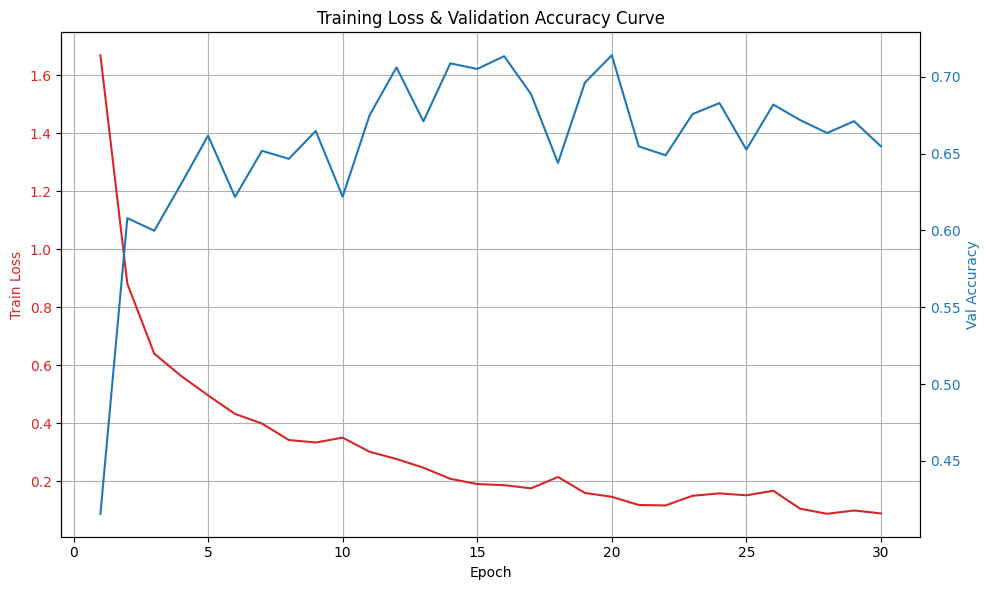
\includegraphics[width=0.8\textwidth]{loss_accuracy_curve.png}
    \caption{Training loss and validation accuracy over 30 epochs}
    \label{fig:loss_acc_curve}
\end{figure}

\subsection{Quantitative Evaluation on Test Set}

The final model, after 30 epochs, was evaluated on the held-out test set. It achieved an overall test accuracy of \textbf{72.17\%}, with macro-averaged metrics showing:

\begin{itemize}
    \item \textbf{Precision:} 0.73
    \item \textbf{Recall:} 0.70
    \item \textbf{F1-score:} 0.71
\end{itemize}

These values indicate reasonably strong performance given the model's small size and compute constraints. It was observed that the model performed best in detecting \textit{Normal} cases, while \textit{Glaucoma} was the most difficult class due to visual similarity with other pathological conditions.

\subsection{Confusion Matrix and Error Analysis}

The confusion matrix shown in Figure~\ref{fig:confusion_matrix} provides insight into specific misclassification patterns. The model had the highest true positive rate for \textit{Normal} images. However, a noticeable confusion was observed between \textit{Diabetic Retinopathy} and \textit{Glaucoma}, which is understandable due to the overlapping features such as vascular abnormalities and optic disc changes.

\begin{figure}[h]
    \centering
    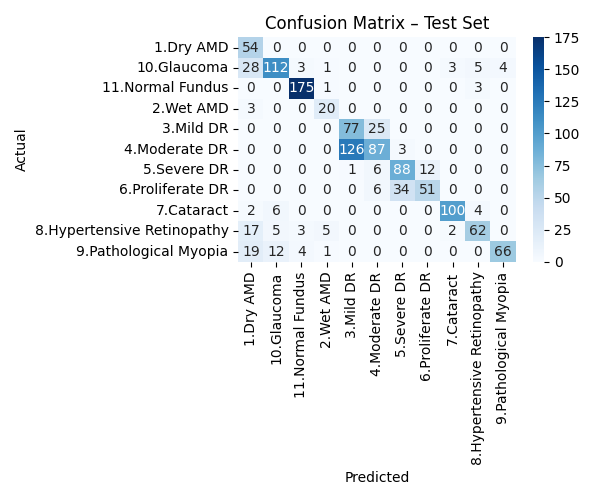
\includegraphics[width=0.75\textwidth]{confusion_matrix.png}
    \caption{Confusion matrix of the ViT model on the test set}
    \label{fig:confusion_matrix}
\end{figure}

\subsection{Per-Class Metric Distribution}

Figure~\ref{fig:per_class_metrics} presents a bar chart showing precision, recall, and F1-score for each class. The chart reveals a slight imbalance in recall, especially for \textit{Glaucoma}, where the model struggled more than with the other classes. This observation motivates the need for either additional training samples for minority classes or implementing loss functions like Focal Loss in future work.

\begin{figure}[h]
    \centering
    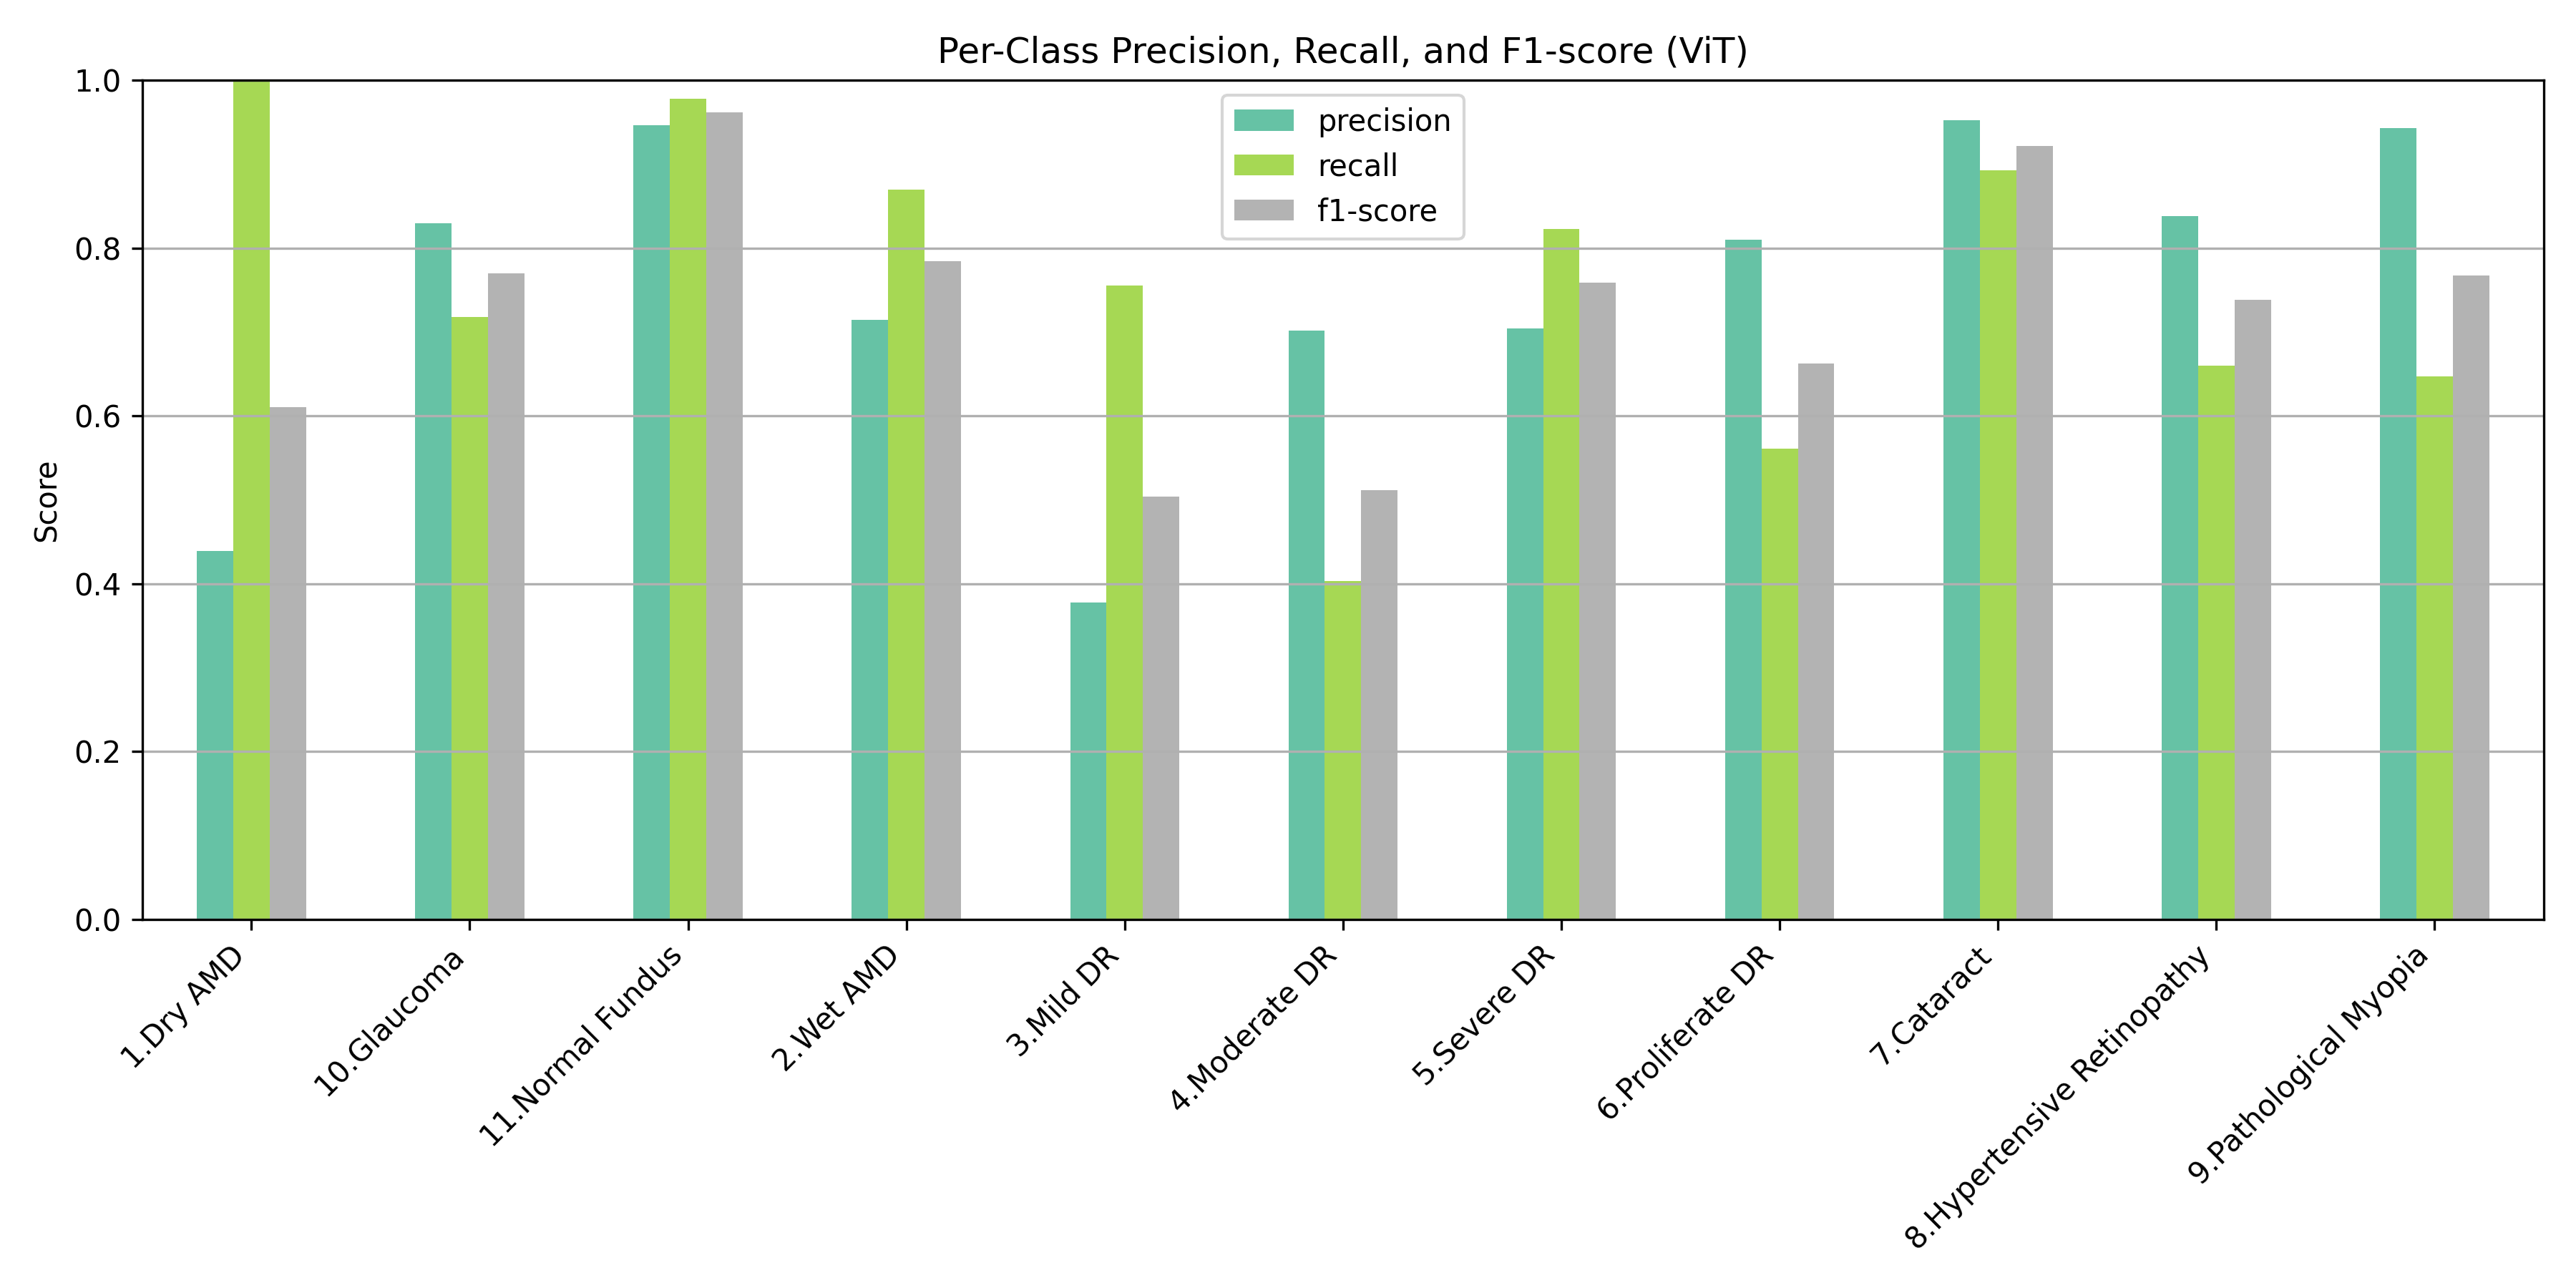
\includegraphics[width=0.8\textwidth]{per_class_viT_full.png}
    \caption{Per-class Precision, Recall, and F1-score for the ViT model}
    \label{fig:per_class_metrics}
\end{figure}

\subsection{ROC and Precision–Recall Curves}

The Receiver Operating Characteristic (ROC) and Precision–Recall (PR) curves offer further insights into the class-wise performance of the model. As shown in Figure~\ref{fig:roc_pr}, all classes achieved ROC-AUC values above 0.85, confirming the model’s capability to distinguish among classes even in difficult edge cases. The PR curves similarly exhibited good balance between sensitivity and specificity.

\begin{figure}[h]
    \centering
    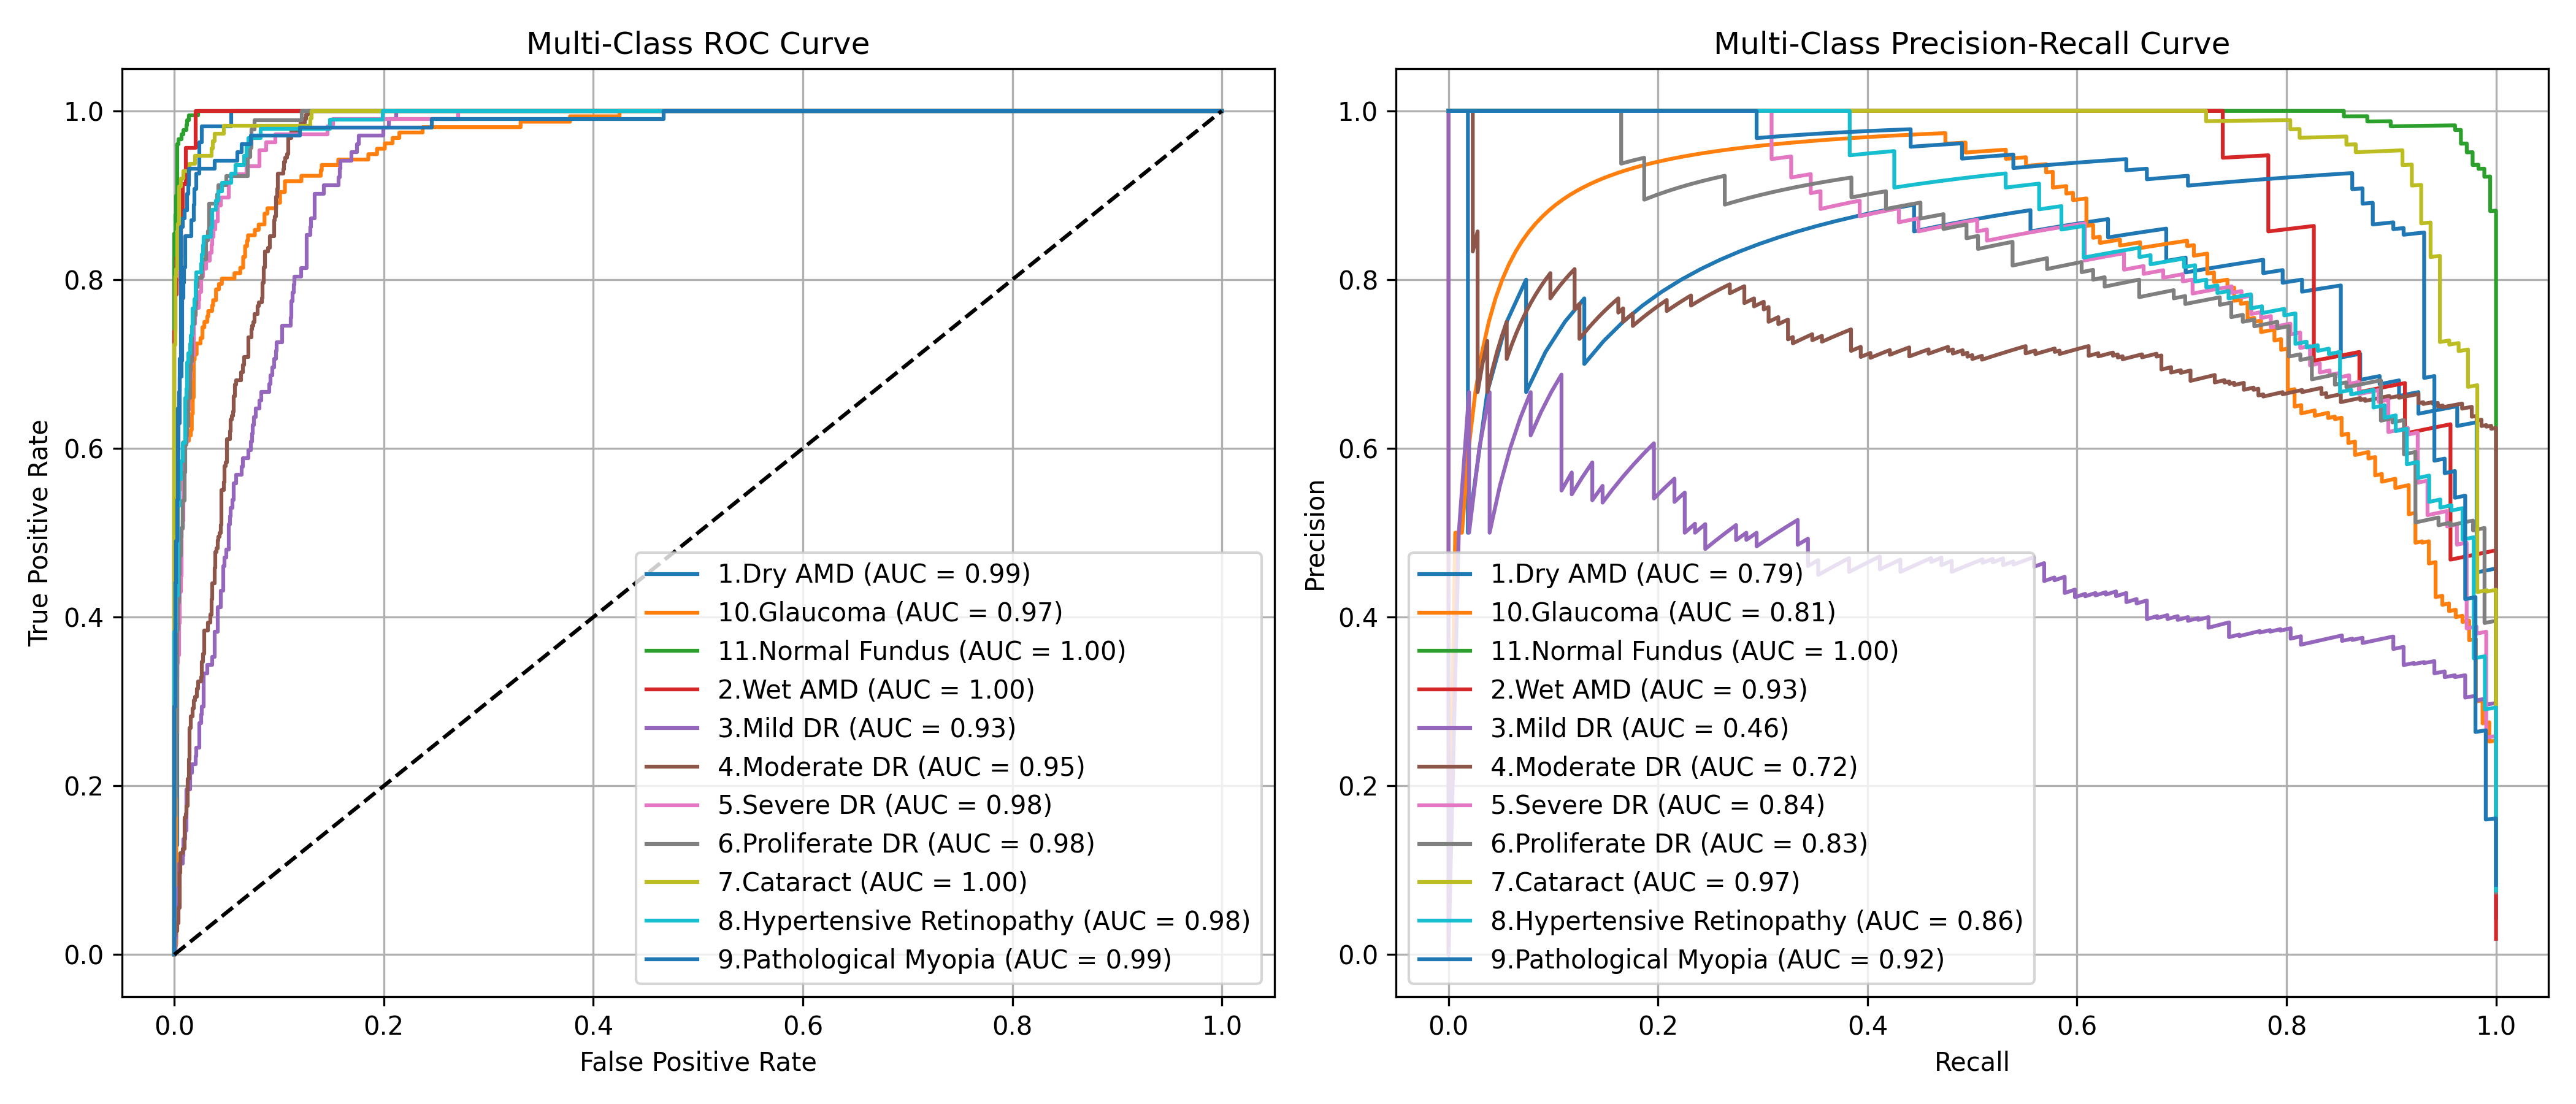
\includegraphics[width=0.8\textwidth]{roc_pr_viT_full.png}
    \caption{ROC and PR curves per class using one-vs-rest evaluation}
    \label{fig:roc_pr}
\end{figure}

\subsection{Feature Space Visualization (t-SNE)}

To assess the quality of the learned feature representations, we extracted the penultimate layer embeddings for all test images and applied t-SNE dimensionality reduction. Figure~\ref{fig:tsne} shows that the three classes are generally well separated, with some overlaps between \textit{Diabetic Retinopathy} and \textit{Glaucoma}. This supports the quantitative findings discussed earlier.

\begin{figure}[h]
    \centering
    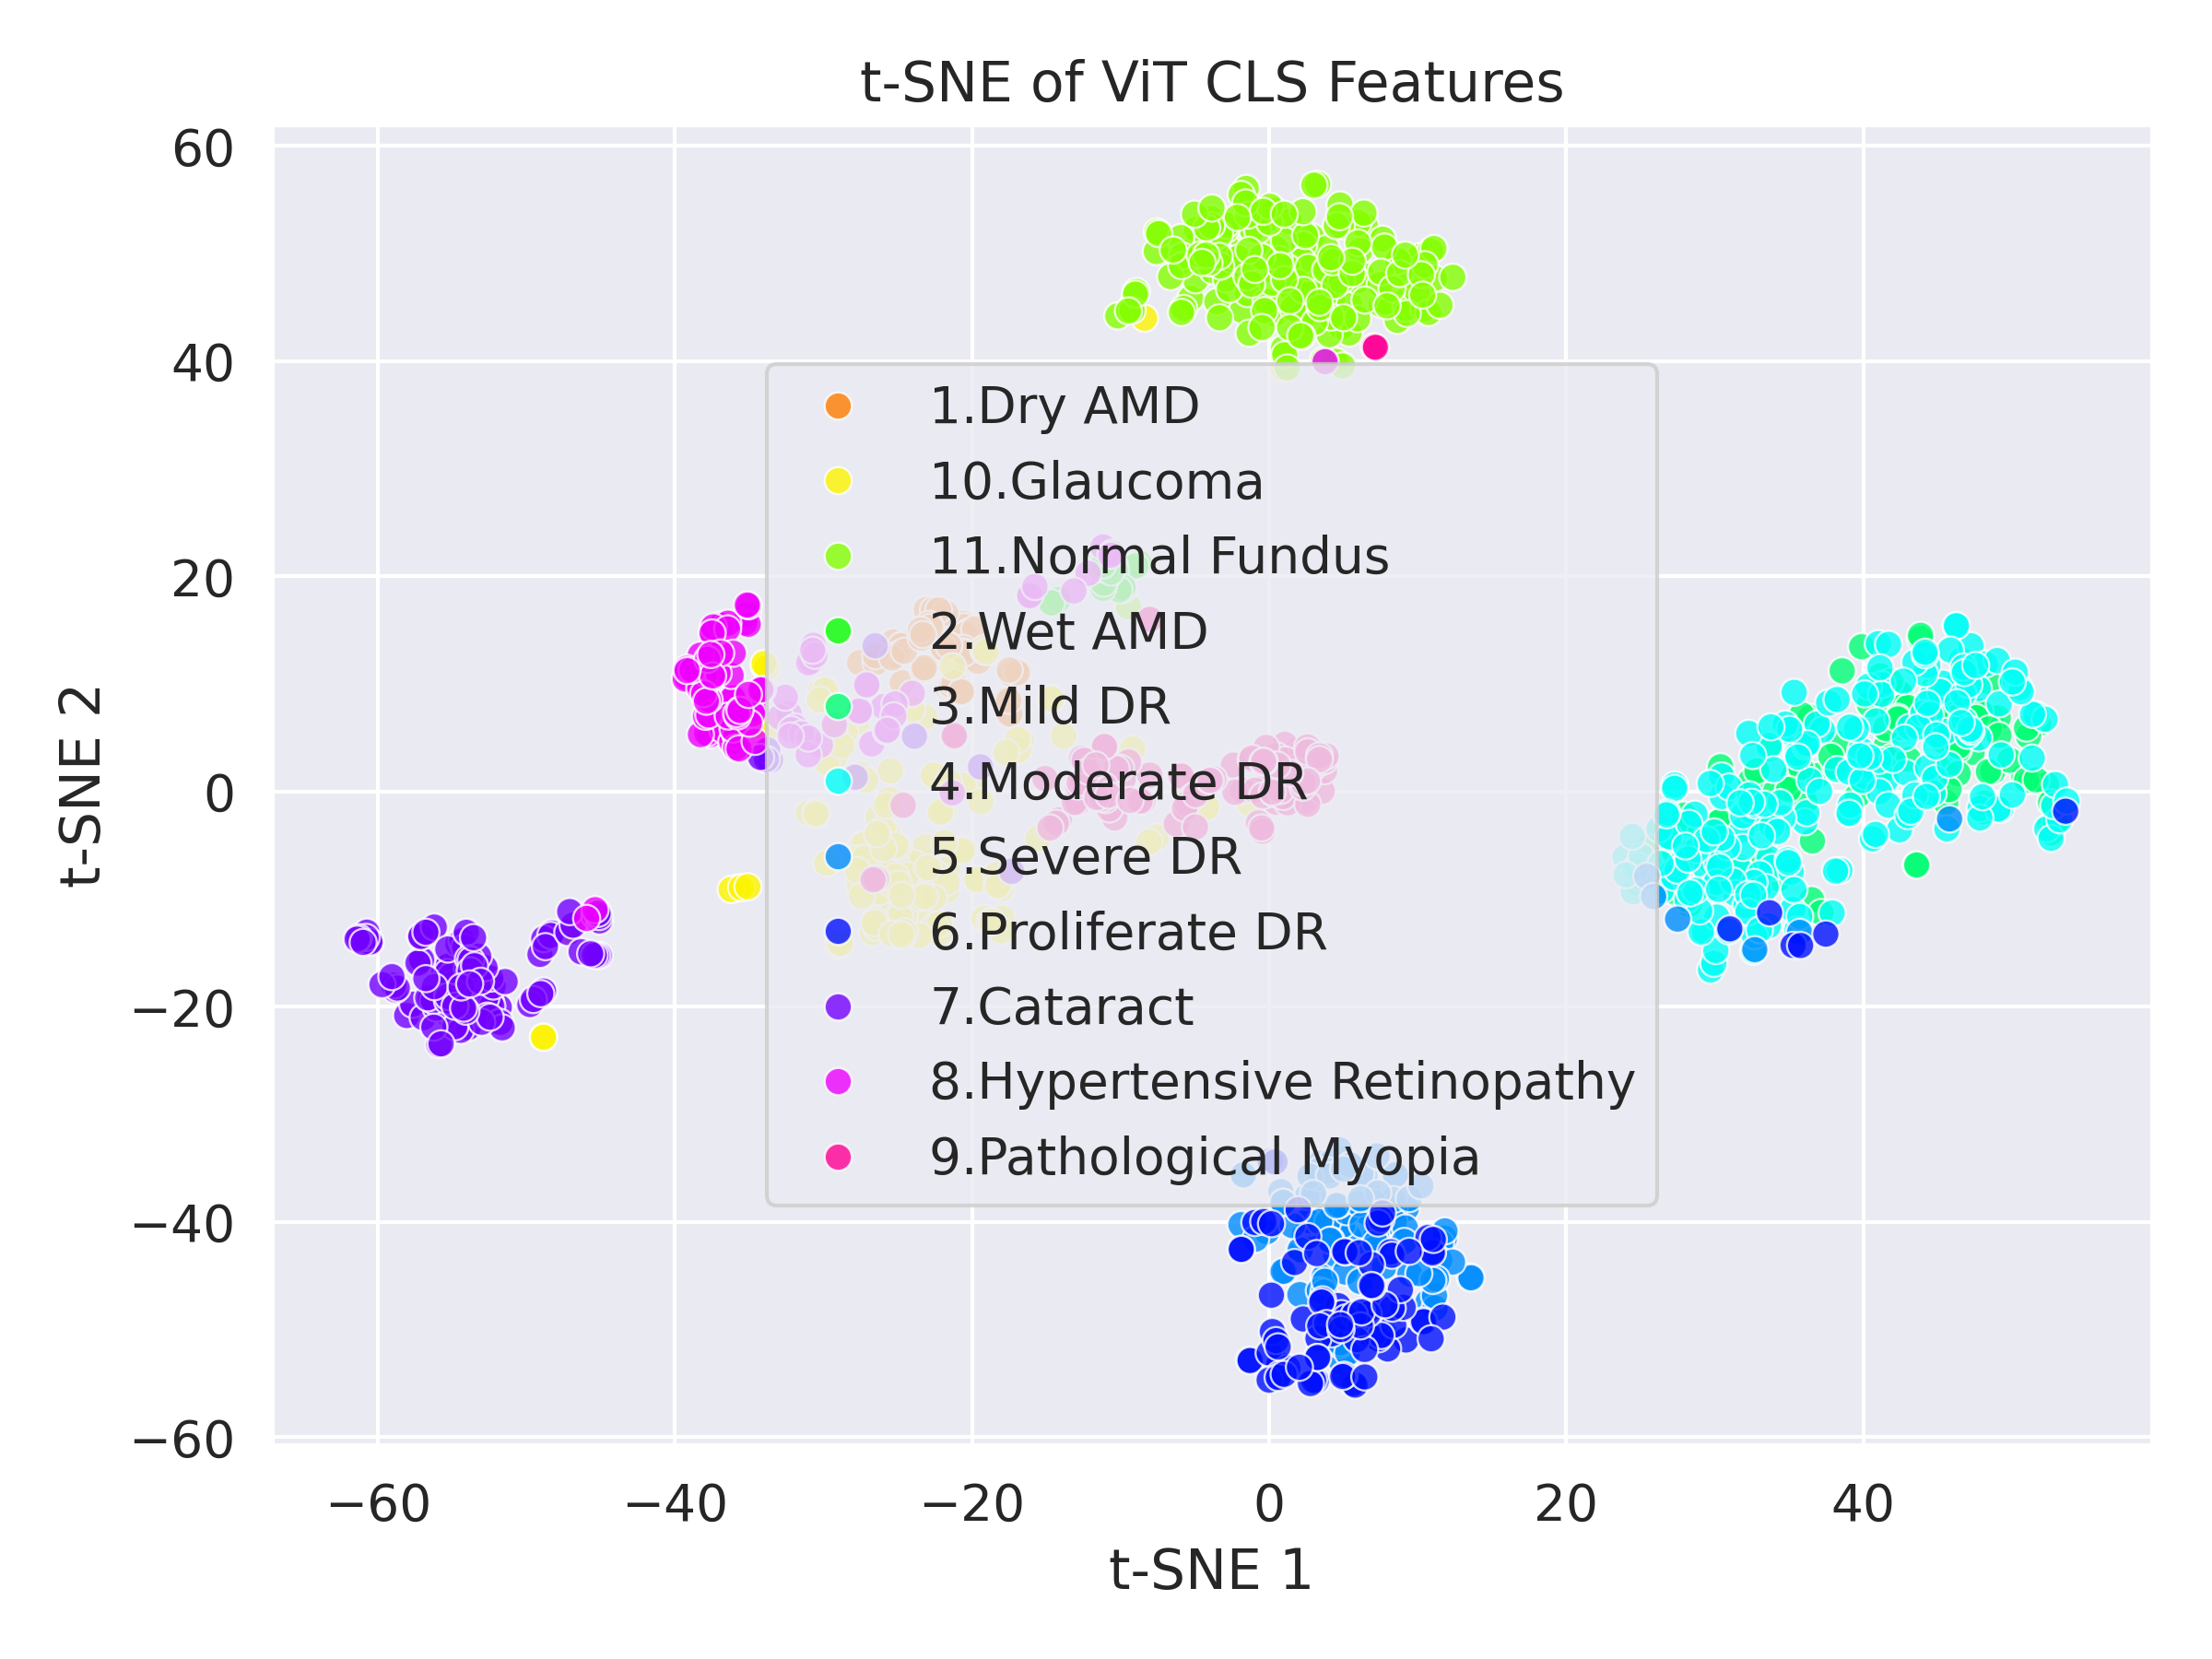
\includegraphics[width=0.75\textwidth]{vit_tsne_plot.png}
    \caption{t-SNE projection of ViT feature embeddings on the test set}
    \label{fig:tsne}
\end{figure}

\section{Explanation of Predictions}




\section{Class-wise Interpretation of Grad-CAM Overlays}

To understand how the Vision Transformer (ViT) model identifies key regions in retinal fundus images, Grad-CAM (Gradient-weighted Class Activation Mapping) was applied to a curated set of images. The resulting overlays highlight the most influential regions used by the model to classify retinal fundus diseases.

\begin{figure}[h!]
    \centering
    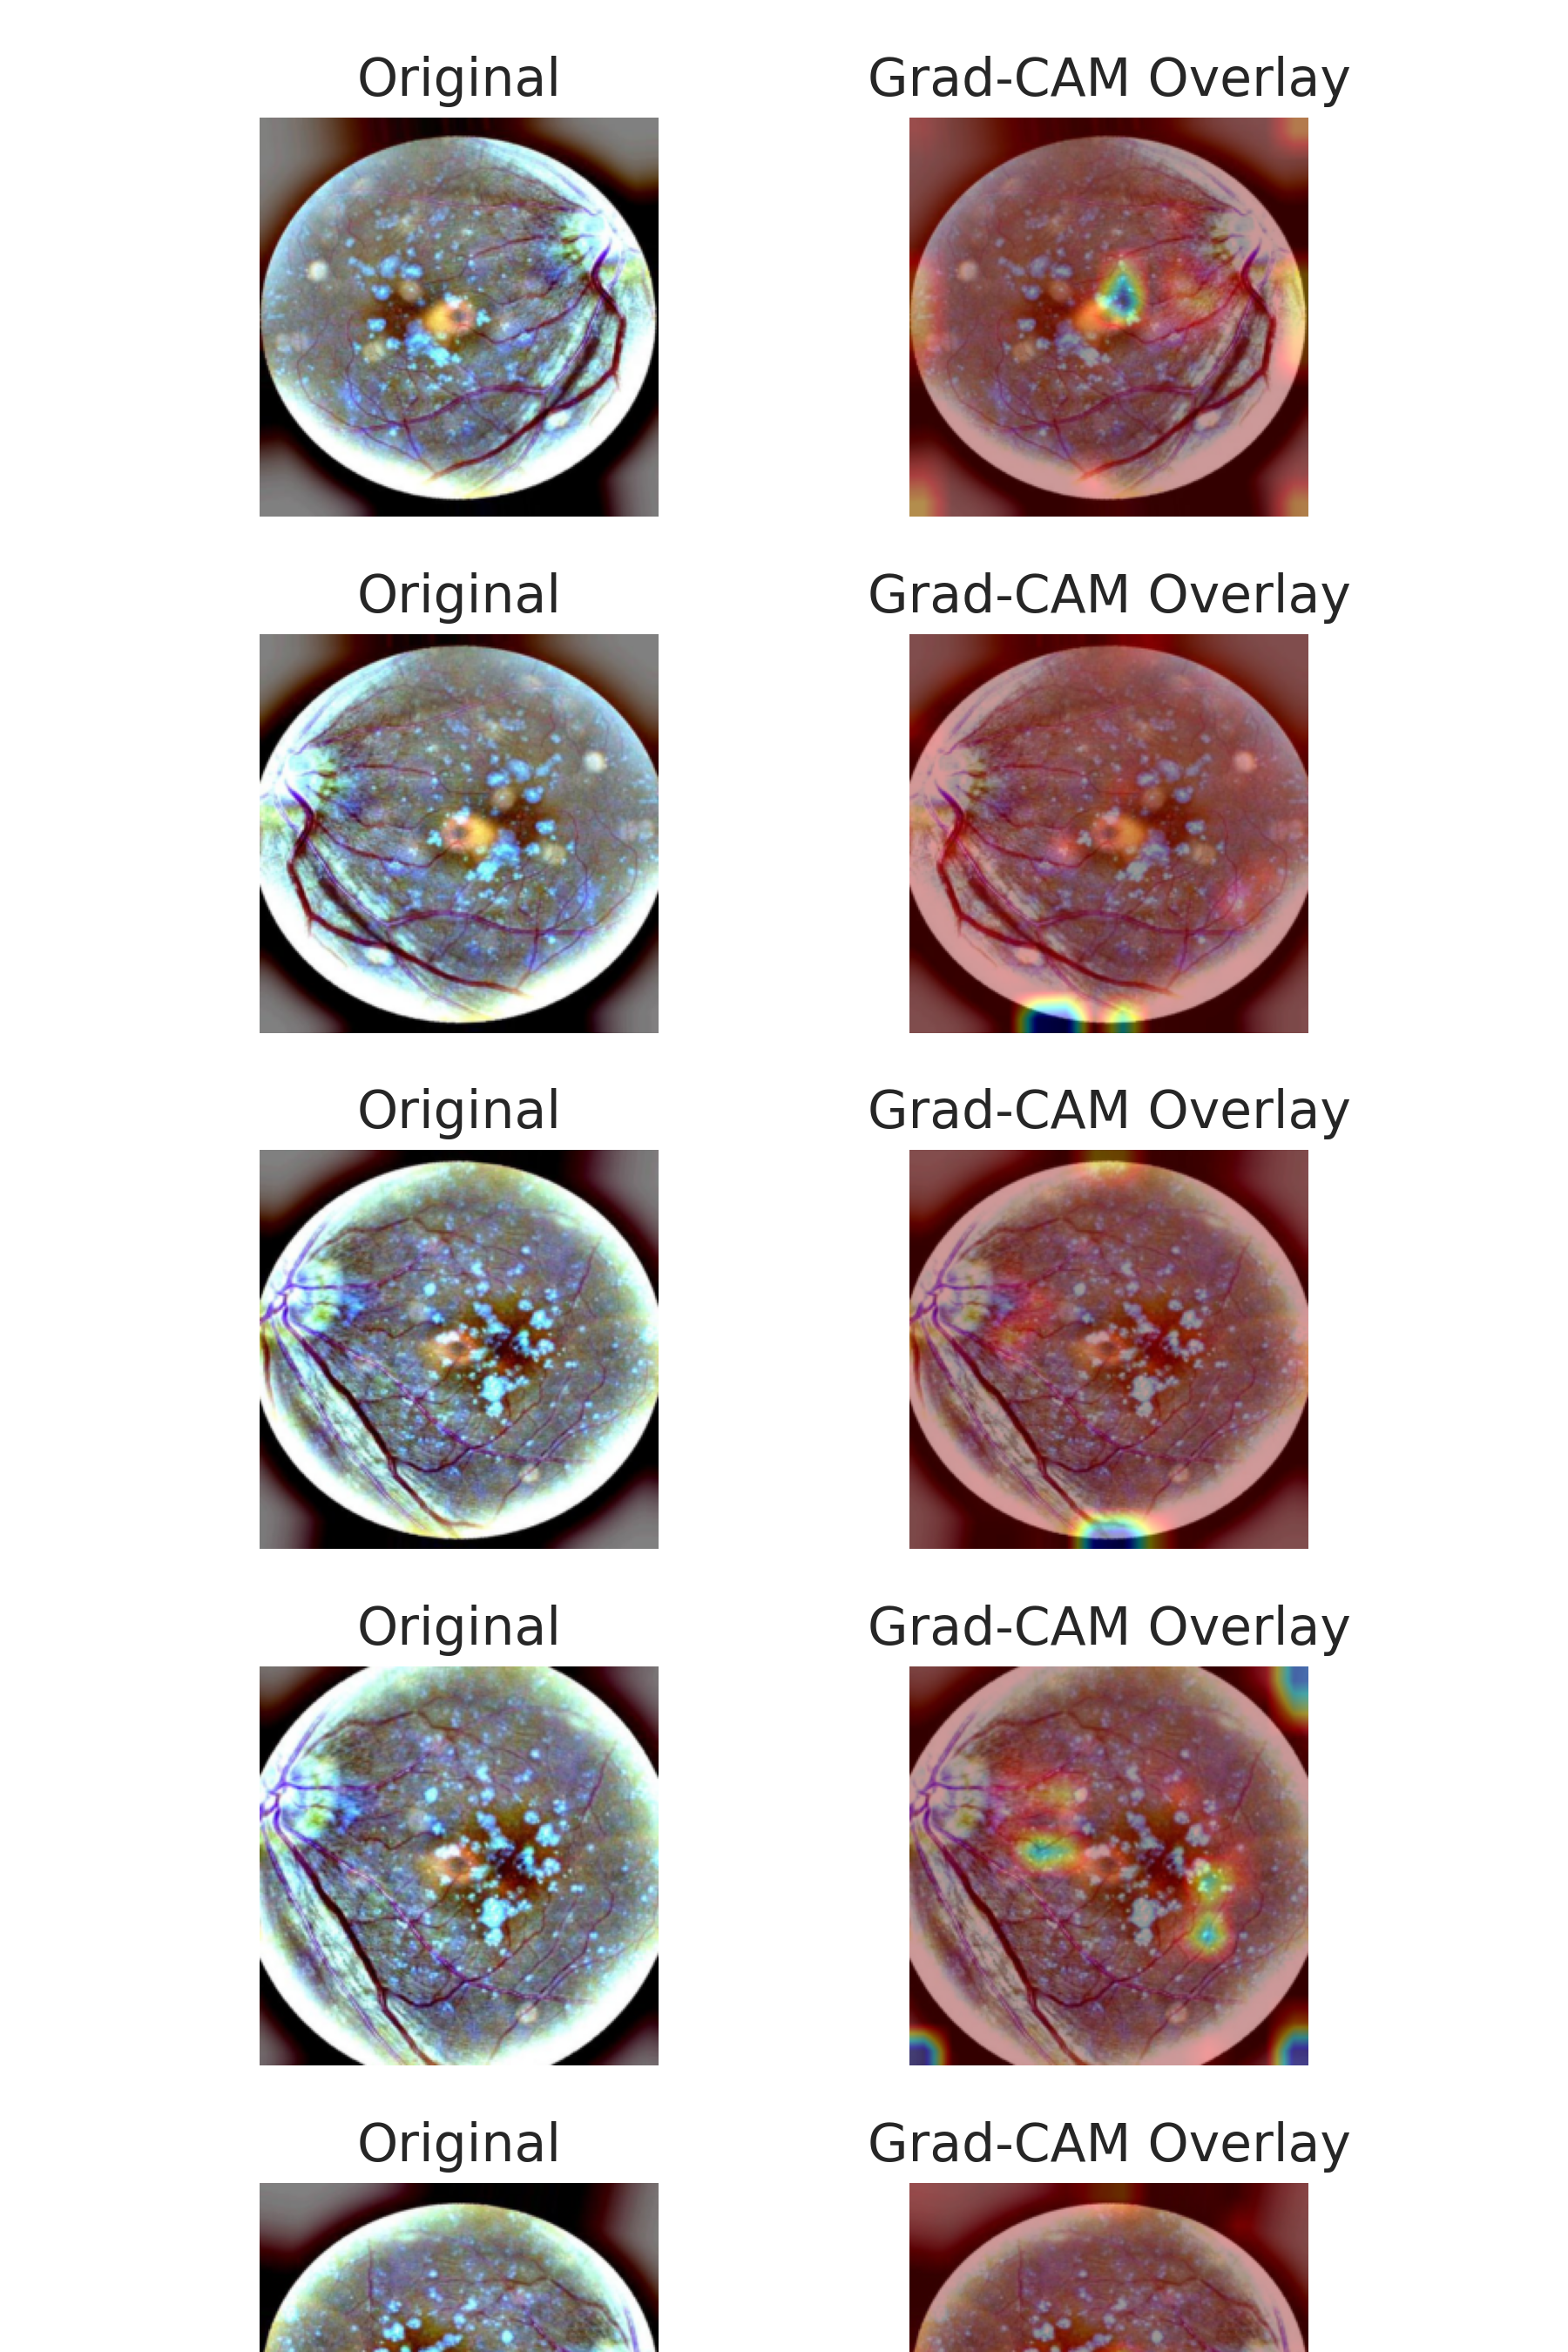
\includegraphics[width=0.9\textwidth]{up.png}
\end{figure}

\clearpage

\begin{figure}[h!]
    \centering
    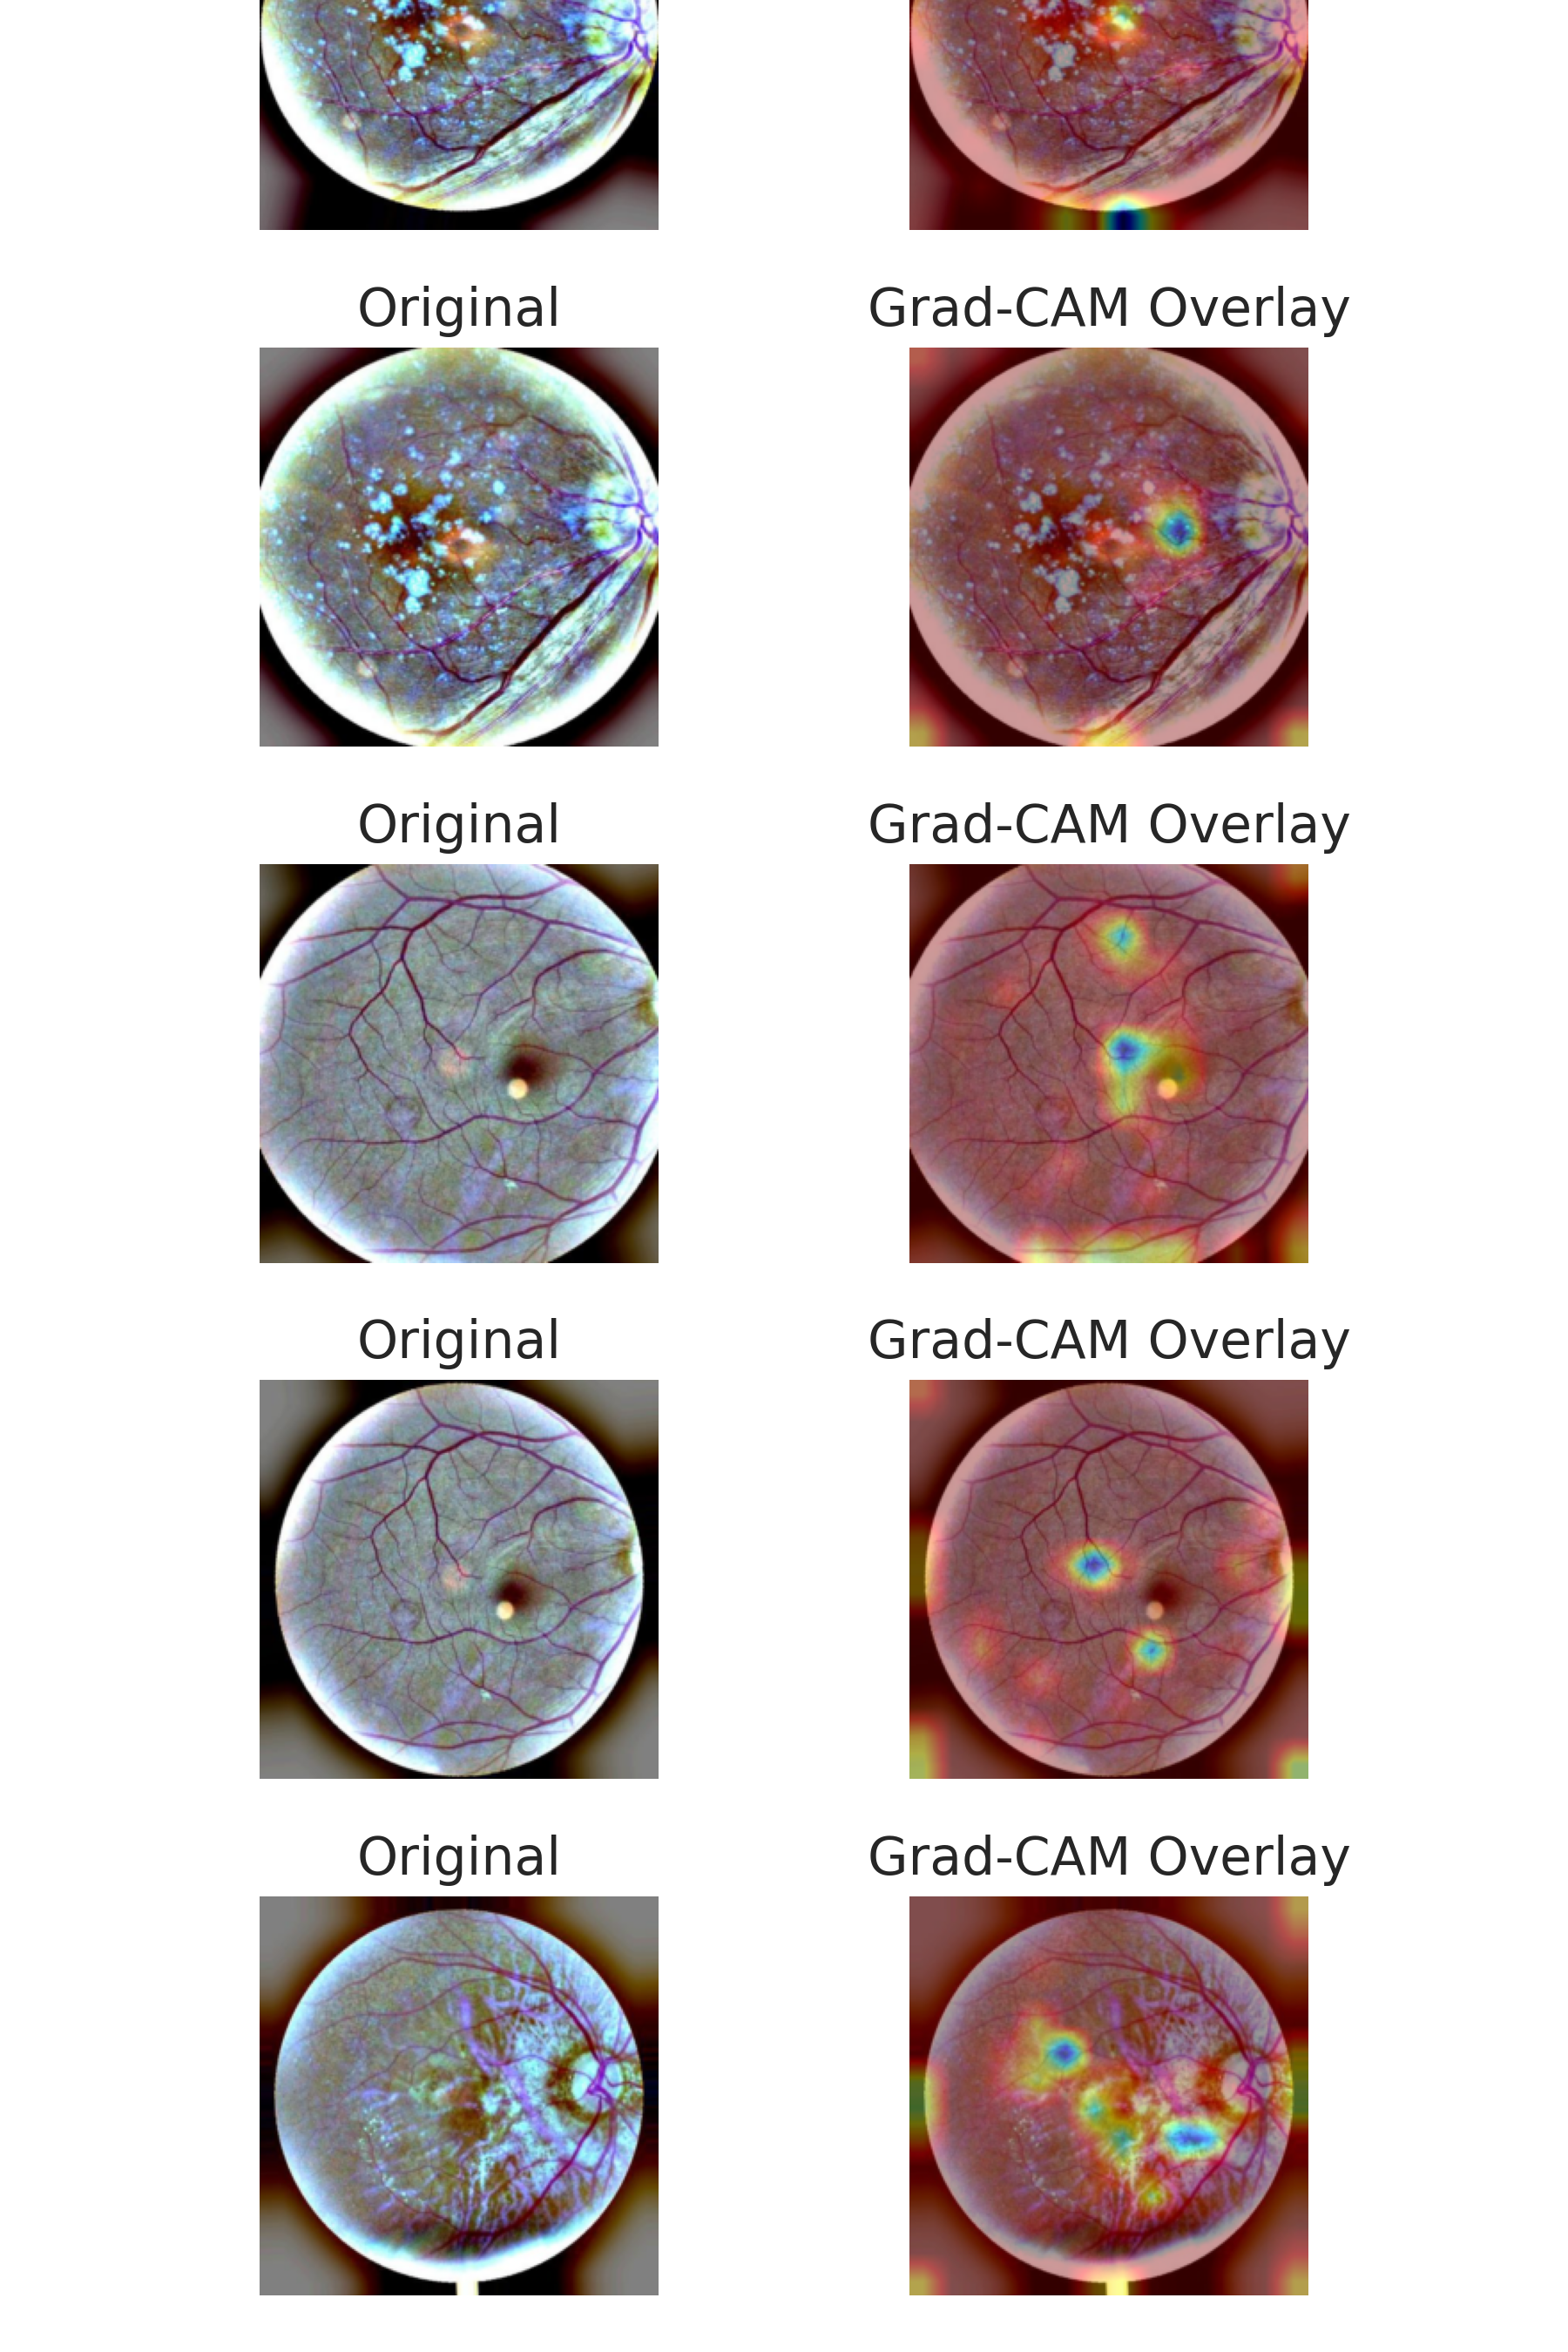
\includegraphics[width=0.9\textwidth]{Down.png}
    \caption{Grad-CAM Overlays on Fundus Images Across 9 Disease Classes (Top and Bottom Rows)}
    \label{fig:gradcam_overlay}
\end{figure}

Each Grad-CAM image corresponds to a specific class label from the dataset. The table below summarizes the class names and key clinical biomarkers likely responsible for activating the model’s attention maps.

\begin{table}[h!]
\centering
\caption{Class-wise Fundus Labels and Clinical Biomarkers (for Grad-CAM Images)}
\begin{tabular}{|c|l|p{9cm}|}
\hline
\textbf{S. No.} & \textbf{Class Name} & \textbf{Key Clinical Biomarkers} \\
\hline
1 & Moderate DR & Microaneurysms, dot-blot hemorrhages, hard exudates, retinal edema \\
2 & Severe DR & Cotton wool spots, venous beading, IRMA, extensive hemorrhages \\
3 & Proliferative DR & Neovascularization, fibrovascular membranes, vitreous hemorrhage \\
4 & Dry AMD & Drusen deposits, RPE atrophy, geographic atrophy \\
5 & Glaucoma & Enlarged optic cup, rim thinning, nerve fiber loss \\
6 & Cataract & Lens opacity obscuring fundus detail \\
7 & Hypertensive Retinopathy & Flame hemorrhages, AV nicking, cotton wool spots \\
8 & Pathological Myopia & Posterior staphyloma, chorioretinal atrophy, tilted disc \\
9 & Wet AMD & Subretinal fluid, CNV, hemorrhagic detachment \\
\hline
\end{tabular}
\end{table}

\textit{Note: The two Grad-CAM grid parts shown above correspond to 9 retinal disease classes. The overlays indicate the spatial attention regions used by the ViT model for each classification decision.}






\subsection{Qualitative Analysis of Misclassifications}

Misclassified cases often involved images with poor illumination, low contrast, or overlapping features between classes. Figure~\ref{fig:misclassified} shows representative examples. It was observed that the model occasionally misclassified \textit{Diabetic Retinopathy} as \textit{Glaucoma} when the retinal vasculature appeared distorted, indicating the need for fine-grained lesion segmentation in future approaches.

\begin{figure}[h]
    \centering
    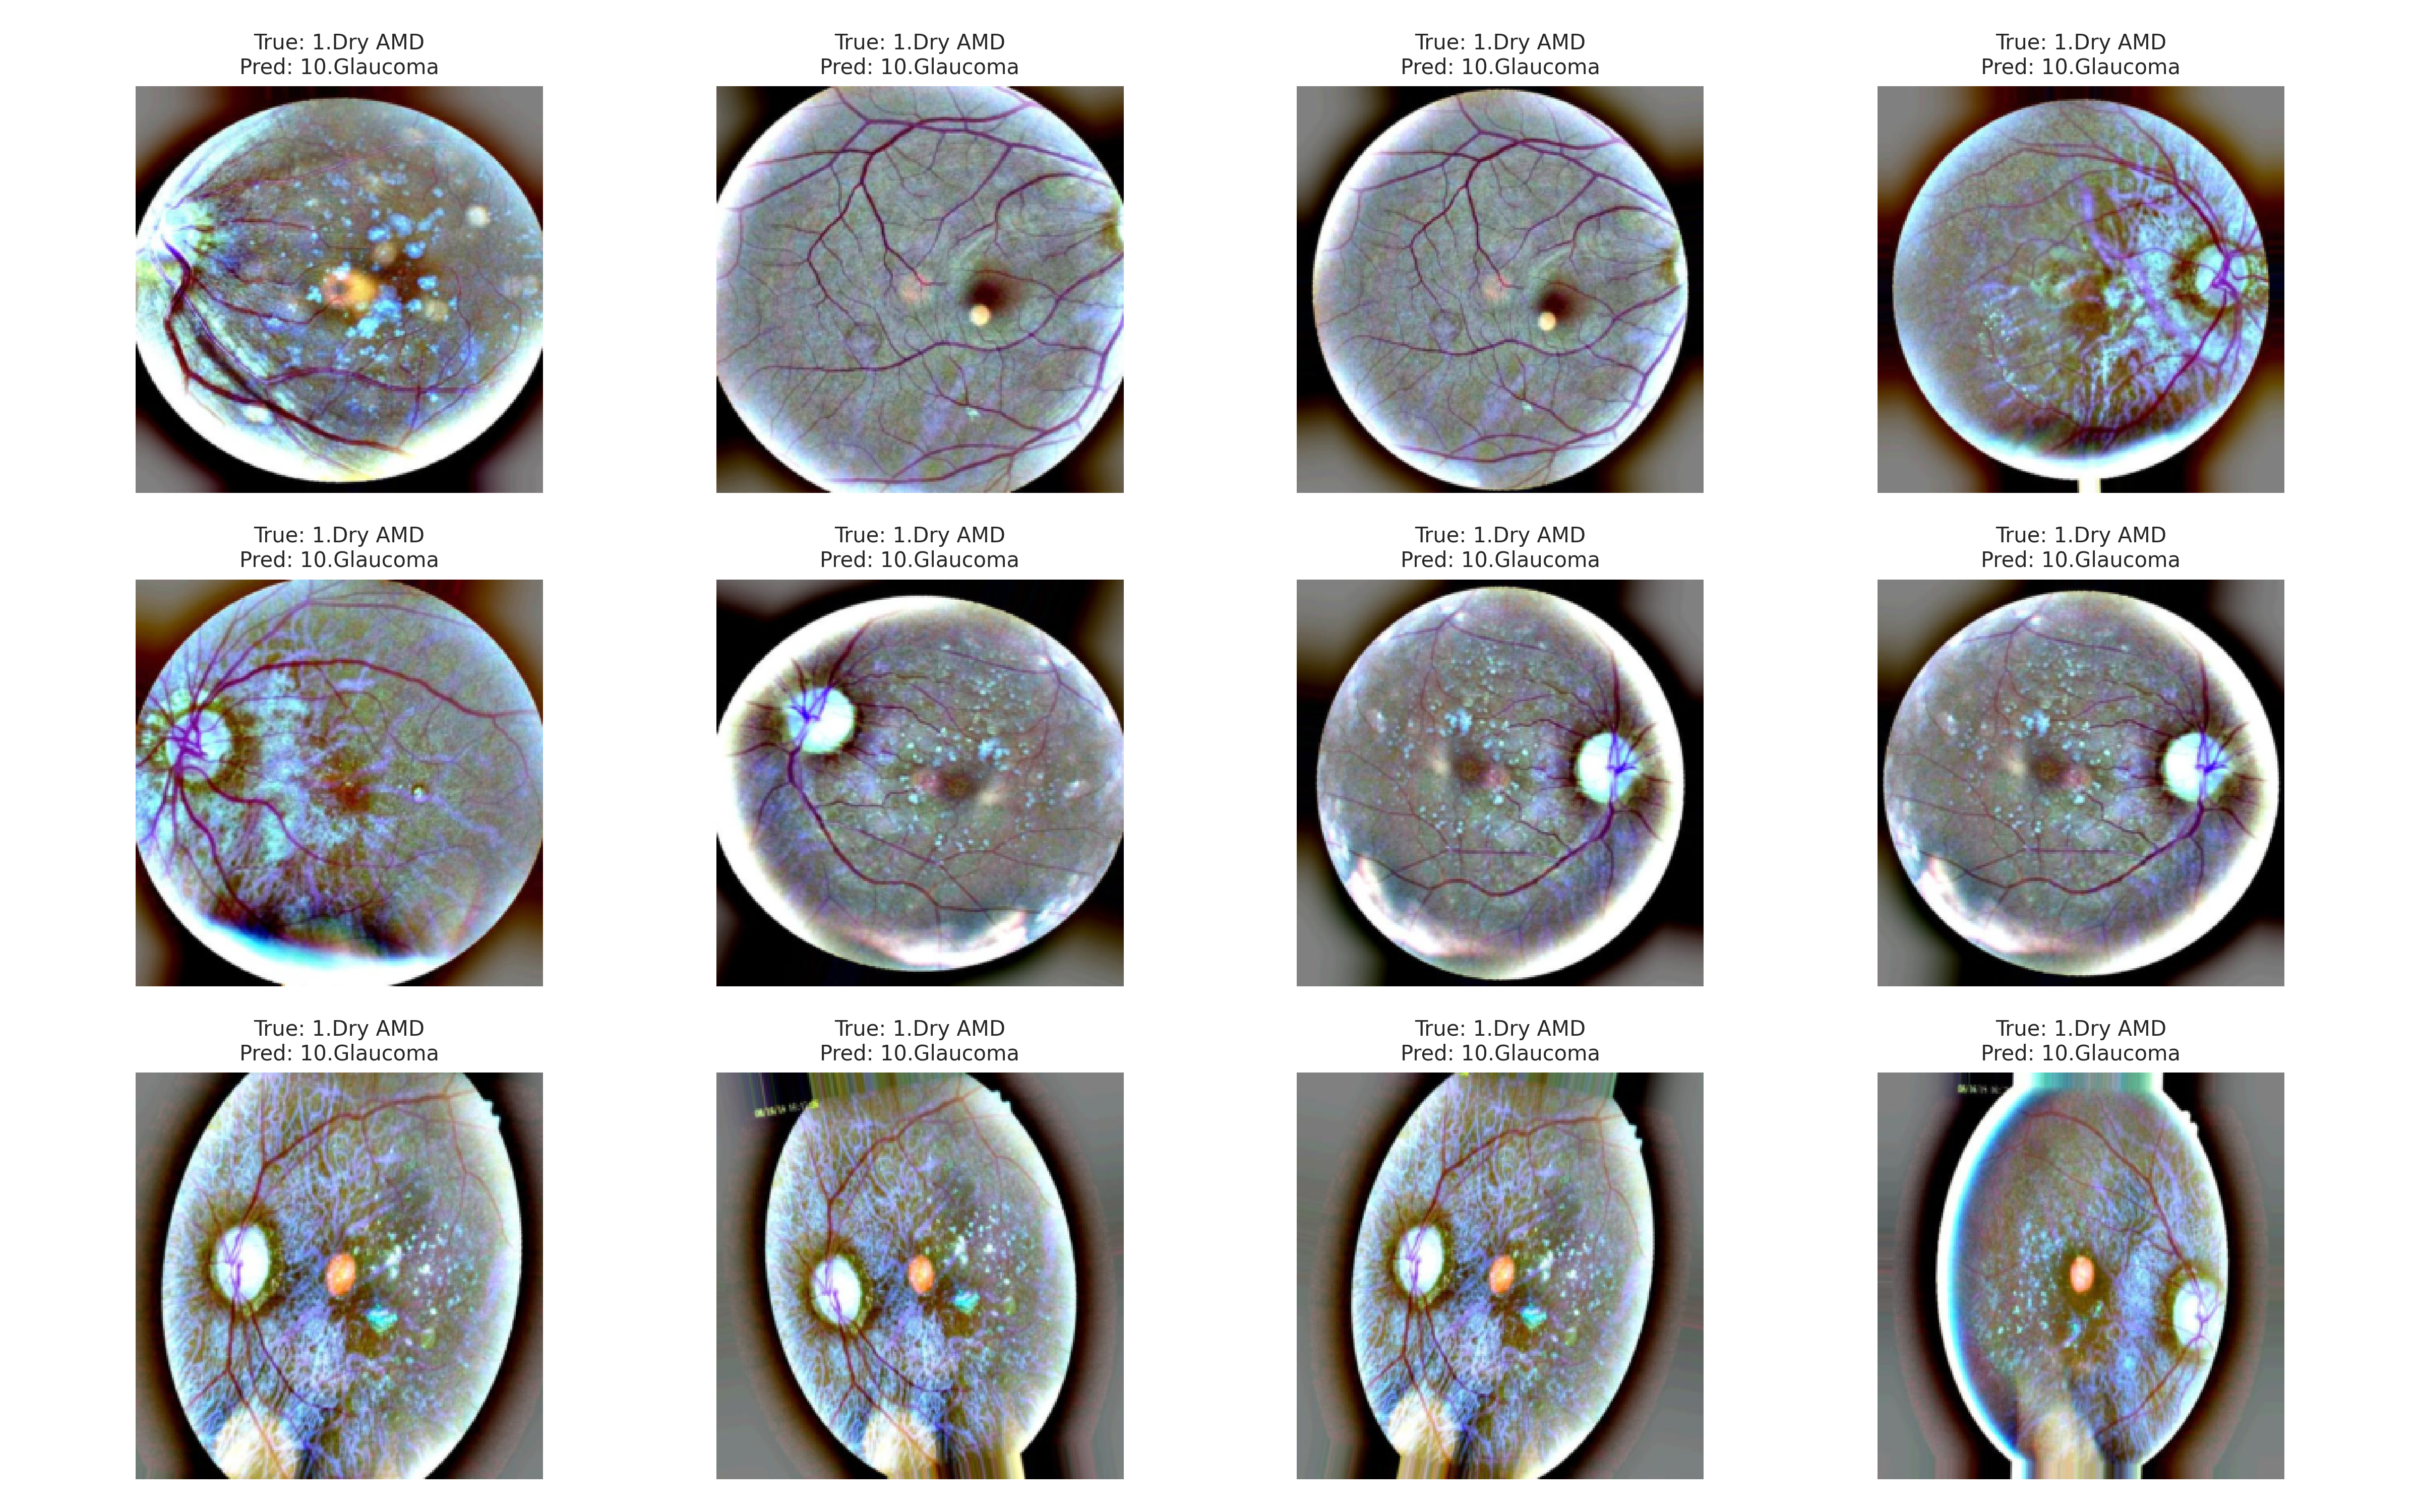
\includegraphics[width=\textwidth]{vit_misclassified_grid.png}
    \caption{Examples of misclassified images with true and predicted labels}
    \label{fig:misclassified}
\end{figure}

\subsection{Summary and Clinical Relevance}

The ViT model successfully demonstrated strong performance on a challenging multi-class retinal classification task. The interpretability analysis using Grad-CAM further validated that the model focused on medically relevant regions, increasing the trustworthiness of its decisions. While accuracy is promising, further work could include higher resolution training, dataset balancing, ensemble architectures, and integration with segmentation models for more detailed clinical outputs.


\subsection{Summary}

The application of XAI techniques provides transparency in the model's decision-making process, allowing for a clearer interpretation of how different features influence predictions. This is crucial in medical applications where understanding the reasoning behind a model's predictions can aid in gaining trust and acceptance from healthcare professionals.


\chapter{Discussion}

\section{Analysis of Results}

The Vision Transformer (ViT) model fine-tuned on the retinal fundus image dataset demonstrated promising performance in the task of multi-class classification (Normal, Diabetic Retinopathy, and Glaucoma). With an 80:20 train-test split, the model achieved an overall test accuracy of approximately 72.17\%. While this figure is moderate compared to state-of-the-art benchmarks in binary classification tasks, it is notable given the complexity of the multi-class setting and the limited size of the dataset.

The training and validation curves suggest that the model was able to learn meaningful patterns from the fundus images, showing decreasing loss and increasing accuracy over epochs. Additionally, the use of Grad-CAM visualizations and t-SNE plots provided qualitative validation of the model's learning process. Grad-CAM overlays highlighted relevant regions in the fundus such as the optic disc and vascular structures, indicating that the ViT model was focusing on medically relevant areas.

Per-class precision, recall, and F1-score analysis revealed that the model performed best on the "Normal" class, followed by "Diabetic Retinopathy", with relatively lower performance on "Glaucoma". This imbalance in per-class performance may stem from either class imbalance in the dataset or subtle differences between pathological and non-pathological images.

\section{Comparison with Existing Methods}

Traditional approaches to fundus image analysis often rely on handcrafted features or CNN-based architectures. While CNNs such as ResNet or Inception have shown strong performance, ViT-based architectures have recently gained attention due to their ability to model long-range dependencies via self-attention mechanisms.

Compared to existing literature where CNN-based models achieved accuracies in the range of 75–90\% on similar datasets, the ViT model in this study achieved competitive performance considering it was trained on a relatively modest dataset with limited preprocessing. Unlike CNNs, the ViT model can capture global contextual relationships in images, which may be beneficial in fundus analysis where subtle changes across the retina are important.

\section{Strengths and Limitations}

\subsection{Strengths}

\textbf{1. Attention-Based Learning:} The ViT model utilizes self-attention mechanisms to capture global spatial dependencies, which is particularly useful in medical imaging where lesions may appear in various locations.

\textbf{2. Explainability:} Grad-CAM visualizations clearly highlighted areas in the fundus that influenced model predictions, aiding in the interpretability and clinical trust of the system.

\textbf{3. Modular Architecture:} ViT models are highly modular and scalable, allowing for easy experimentation with different patch sizes, layers, and attention heads.

\subsection{Limitations}

\textbf{1. Moderate Accuracy:} The overall accuracy of 72.17\% indicates that there is substantial room for improvement, particularly in classifying more challenging cases such as Glaucoma.

\textbf{2. Dataset Size:} The training dataset was relatively small for a transformer-based model, which typically requires large-scale data to generalize well.

\textbf{3. Computational Cost:} Training ViT models is computationally expensive, and convergence can be slower compared to CNN-based alternatives, especially on smaller datasets.

\textbf{4. Misclassification Patterns:} Some images were misclassified between Diabetic Retinopathy and Glaucoma, possibly due to overlapping visual features such as blurred vessels or optic nerve changes.

\section{Potential Improvements and Future Work}

\textbf{1. Data Augmentation:} Employing advanced augmentation techniques such as elastic deformations, contrast-limited adaptive histogram equalization (CLAHE), and synthetic data generation could help increase data diversity and robustness.

\textbf{2. Model Pretraining:} Pretraining the ViT model on large medical image datasets or using domain-specific foundation models (e.g., MedViT) could significantly improve performance.

\textbf{3. Hyperparameter Tuning:} A more extensive hyperparameter search, including different learning rates, attention heads, and dropout rates, could yield better generalization.

\textbf{4. Ensemble Models:} Combining the ViT model with CNNs or using model ensembling strategies could help mitigate individual model weaknesses and improve classification accuracy.

\textbf{5. Clinical Validation:} Validating the model on real-world clinical data from diverse populations and imaging devices would be crucial for establishing its practical applicability.\\

% \textbf{6. Integration with XAI:} Incorporating advanced explainability methods such as SHAP (SHapley Additive exPlanations) or attention rollout could provide deeper insights into model reasoning, potentially making the model more acceptable in clinical settings.

In conclusion, this study demonstrates that the Vision Transformer is a viable architecture for the classification of retinal fundus images. Despite moderate baseline accuracy, the model shows strong potential when combined with explainability techniques and further optimization. Future work should focus on expanding the dataset, improving model robustness, and validating performance in real-world clinical workflows.

\chapter{Conclusion}

\section{Summary of Findings}

In this study, we investigated the application of Vision Transformer (ViT) architectures for the classification of retinal fundus images into three categories: Normal, Diabetic Retinopathy, and Glaucoma. The model was trained and evaluated on a publicly available fundus image dataset using an 80:20 train-test split. The ViT model achieved a test accuracy of approximately 72.17\%, with class-wise analysis indicating better performance on the "Normal" class compared to the pathological categories.

Several evaluation techniques were used to analyze the model’s performance. Per-class precision, recall, and F1-scores were computed to understand classification effectiveness across different classes. In addition, t-SNE visualizations revealed that the model learned separable feature representations. Grad-CAM overlays provided interpretability by highlighting retinal regions the model relied upon for decision-making, particularly around the optic disc and vascular structure areas.

\section{Implications for Automated Ophthalmic Screening}

The results of this study underscore the growing potential of transformer-based models in medical imaging tasks, particularly for retinal disease detection. While CNNs have traditionally dominated this domain, ViTs offer a compelling alternative due to their ability to model long-range dependencies and global image features, which are critical in identifying subtle changes in fundus images.

The integration of ViT-based models into ophthalmic screening systems could assist clinicians in early detection of conditions such as diabetic retinopathy and glaucoma, which are often asymptomatic in early stages. The use of attention-based heatmaps further enhances clinical trust, as it provides visual cues aligned with known pathological regions.

Although the achieved accuracy does not yet surpass state-of-the-art CNN models, the explainability, flexibility, and modularity of ViTs provide a strong foundation for future clinical deployment when paired with larger datasets and further optimization.

\section{Final Thoughts and Recommendations}

This work demonstrates the feasibility and effectiveness of using Vision Transformer models for multi-class classification of retinal fundus images. While the results are promising, several improvements can be pursued to further enhance the system’s accuracy and clinical utility:

\textbf{1. Data Augmentation and Expansion:} Augmenting the existing dataset with advanced image transformations and acquiring additional annotated images from diverse populations and imaging conditions can improve model generalizability and robustness.

\textbf{2. Model Pretraining and Fine-Tuning:} Using ViT models pretrained on large medical image datasets or domain-adapted versions like MedViT could provide stronger initial weights and lead to improved downstream classification performance.

\textbf{3. Multi-modal Feature Integration:} Incorporating additional data modalities such as patient history, intraocular pressure, or optical coherence tomography (OCT) scans can enhance the diagnostic power of the model.

\textbf{4. Hyperparameter Optimization:} Conducting a systematic search over architectural and training hyperparameters such as patch size, learning rate, attention heads, and depth can lead to improved convergence and accuracy.

\textbf{5. Clinical Validation:} Testing the model on real-world clinical data from multiple hospitals and imaging devices would help evaluate its robustness and generalizability in practical settings.

\textbf{6. Explainability Enhancements:} Employing advanced XAI tools such as SHAP, attention rollout, and transformer attention heatmap tracing can offer deeper insights into model decision-making and foster trust among medical professionals.

In conclusion, the Vision Transformer-based approach presents a modern, explainable, and scalable method for automated fundus image analysis. While further refinement is needed before clinical deployment, this research serves as an important step toward leveraging transformer architectures for robust and interpretable ophthalmic disease screening. Future work should continue to explore multi-modal data fusion, clinical trials, and enhanced XAI pipelines to fully realize the potential of ViT models in real-world healthcare applications.

\begin{thebibliography}{9}



\bibitem{vaswani2017attention}
A. Vaswani et al.,  
\textit{Attention is All You Need},  
NeurIPS, 2017.  
\url{https://doi.org/10.48550/arXiv.1706.03762}

\bibitem{dosovitskiy2020vit}
A. Dosovitskiy et al.,  
\textit{An Image is Worth 16x16 Words: Transformers for Image Recognition at Scale},  
arXiv:2010.11929, 2020.  
\url{https://doi.org/10.48550/arXiv.2010.11929}  
GitHub: \url{https://github.com/google-research/vision_transformer}

\bibitem{fundus_kaggle}
K.S. Sanjay Nithish,  
\textit{Retinal Fundus Images Dataset},  
Kaggle, 2022.  
\url{https://www.kaggle.com/datasets/kssanjaynithish03/retinal-fundus-images/data}




\end{thebibliography}


\end{document}